\documentclass[11pt,a4paper]{tesis}

\usepackage{thesis}
\usepackage{sections/nd_rules}

\usepackage{fancyhdr}
\pagestyle{fancy}

\usepackage[left=3cm,right=3cm,bottom=3.5cm,top=3.5cm]{geometry}

\usepackage[dvipsnames]{xcolor} % \textcolor
\usepackage[colorlinks=true]{hyperref}  % referencias

\newtheorem{theorem}{Teorema}
\newtheorem*{theorem*}{Teorema}

\newtheorem{corollary}{Corolario}
\newtheorem*{corollary*}{Corolario}

\newtheorem{lemma}{Lema}
\newtheorem*{lemma*}{Lema}

\newtheorem{definition}{Def.}
\newtheorem*{definition*}{Def}


% Para solo agregar algunas secciones
% \includeonly{
%     sections/intro,
%     sections/natural_deduction,
%     sections/ppa,
%     sections/ppa_certifier
% }

\begin{document}
%%%% CARATULA

\def\autor{Manuel Panichelli}
\def\tituloTesis{
PPA - Un asistente de demostración para lógica de primer orden con extracción de
testigos usando la traducción de Friedman
}
\def\runtitulo{PPA - Un asistente de demostración para lógica de primer orden
con extracción de testigos usando la traducción de Friedman}
\def\runtitle{PPA - a proof-assistant for first-order logic with witness extraction using Friedman's translation}
\def\director{Pablo Barenbaum}
\def\lugar{Buenos Aires, 2024}

\input{caratula}

\frontmatter
\pagestyle{empty}
%\begin{center}
%\large \bf \runtitulo
%\end{center}
%\vspace{1cm}
\chapter*{\runtitulo}

\noindent Los \textit{asistentes de demostración} son programas que facilitan la
escritura de demostraciones matemáticas, que pueden ser usados para
facilitar la colaboración masiva o hacer verificación formal de programas. Existen muchos asistentes como Mizar, Coq e Isabelle, basados en distintas teorías. Un criterio deseable que pueden cumplir es el de De Bruijn: a partir de demostraciones en su lenguaje se pueden extraer otras más elementales, que puedan ser chequeados por un programa independiente.

En esta tesis se presenta PPA, un asistente de demostración para lógica clásica
de primer orden. Cumple con el criterio de De Bruijn, generando
demostraciones en el sistema lógico de \textit{deducción natural} a partir de
demostraciones escritas en un lenguaje de alto nivel, cuyo objetivo es ser
similar a cómo serían escritas en lenguaje natural. Tiene un mecanismo principal
de demostración, el by, que por debajo cuenta con un \textit{solver} heurístico
para lógica de primer orden que facilita la escritura de demostraciones. Está
inspirado en el mecanismo análogo en Mizar.

Algunos asistentes implementan la \textit{extracción de testigos de
existencial}. Dada una demostración de $\exists \var . \pred(\var)$, se extrae
un \textit{testigo} $\term$ tal que cumpla $\pred(\term)$. Es sencillo hacerlo sobre lógica intuicionista, pues es constructiva, pero un desafío sobre lógica clásica, que no lo es. Para ello hay dos grandes categorías: directas (mediante semántica operacional de cálculos $\lambda$ clásicos, como realizabilidad clásica) o indirectas (mediante traducciones a lógica intuicionista o similares).

PPA implementa la extracción de forma indirecta usando la traducción de
Friedman, que permite traducir demostraciones clásicas de fórmulas $\classPiTwo$
de la forma $\forall \varTwo_0 \dots \forall \varTwo_n . \exists \var .
\anyForm$ a intuicionistas. Se describe cómo pueden ser normalizadas usando
reglas de reducción bien conocidas, isomorfas a la semántica operacional del cálculo lambda vistas desde el isomorfismo Curry-Howard. Finalmente, de una demostración normalizada se podrá extraer un testigo.
Identificamos algunos detalles en la implementación práctica de la traducción,
que limitan las fórmulas para las cuales se puede usar (más allá de la
limitación teórica de $\classPiTwo$) y también limitan las axiomatizaciones de
las teorías que se pueden hacer.

\bigskip

\noindent\textbf{Palabras claves:} asistente de demostración, lógica de primer orden, deducción natural, lógica clásica, lógica intuicionista, extracción de testigos, traducción de Friedman.

\cleardoublepage
%\begin{center}
%\large \bf \runtitle
%\end{center}
%\vspace{1cm}
\chapter*{\runtitle}

\noindent \textit{Proof assistants} are programs that simplify the writing of
mathematical proofs, enabling large-scale collaboration or the formal
verification of programs. There are many proof assistants such as Mizar, Coq,
and Isabelle, based on different theories. A desirable property they may have is
described by the De Bruijn criterion: from proofs written in a high level
language, one can extract proofs in a core, easily verifiable language. This
eliminates the need to trust their implementation, as the extracted proofs can
be verified by an independent program.

This thesis presents \textit{PPA}, a proof assistant for classical first-order logic. It fulfills De Bruijn's criterion by generating proofs in the natural deduction proof system from high-level proofs, designed to resemble natural language as closely as possible. Its main proof mechanism, \texttt{by}, features an underlying heuristic solver for first-order logic, inspired by Mizar's analogous mechanism.

Some proof assistants implement \textit{existential witness extraction}. Given a
proof of $\exists \var . \pred(\var)$, they extract a *witness* \( \term \) such
that \( \pred(\var) \) holds. While this is straightforward in intuitionistic
logic due to its constructive nature, it is challenging in classical logic,
which lacks constructiveness. There are two main approaches: direct (using
semantic techniques such as classical realizability \cite{miquel-friedman}) or indirect
(via translations to another logic, such as intuitionistic).

The main contribution of this work is a practical implementation of witness
extraction. PPA achieves this indirectly by using Friedman's translation, which
allows converting classical proofs of \( \classPiTwo \) formulas of the form \(
\forall y_0 \dots \forall y_n . \exists x . \anyForm \), with the formula
$\anyForm$ having no quantifiers, into intuitionistic ones. We
describes how, once translated, these proofs can be normalized using well-known
reduction rules, which correspond to the reduction rules of lambda calculus viewed through the Curry-Howard isomorphism. Finally, a
normalized proof enables the extraction of a witness. We identify some practical
implementation details of the translation, which limit the formulas for which it
can be used (beyond the theoretical \( \classPiTwo \) restriction) and also
constrain the axiomatizations of theories that can be made.

\bigskip

\noindent\textbf{Keywords:} proof assistant, first-order logic, natural deduction, classical logic, intuitionistic logic, witness extraction, Friedman's translation.

\cleardoublepage
\chapter*{Agradecimientos}

\noindent 

A mi director, Pablo, por toda su ayuda y paciencia a lo largo de estos años y
por traerme un tema de tesis que era justo lo que buscaba. Gracias a \todo{[nombre1]} y \todo{[nombre2]} por brindar su tiempo para ser jurados en esta tesis.

A mi viejo, por inculcarme la importancia de tener una formación universitaria.

A mi vieja, por acompañarme durante toda la cursada, bancando mis largas tardes
de estudio y esperándome con la comida los días que volvía a las 10 de la noche.

A mis amigos y compañeros de cursada que me acompañaron toda la carrera: Elias,
Gasti, las Guadas, Giampa, Nacho, Tropi, Vladi, Ale, Bruno, Gabi, Juli, Octo,
Schuster y Delgado. Sin ustedes, no hubiera llegado hasta acá.

A Jessi por acompañar los momentos estresantes del último tiempo, y enseñarme el
valor de relajar y no estar siempre desbordado con cosas.

A mis docentes, de la secundaria Chamo que me convenció de estudiar esta
hermosa carrera, y los de la carrera por inspirarme a seguir adelante. Gracias a
mis alumnos y alumnas por permitirme dar al menos un poco de lo que recibí, y
gracias a la Universidad pública por hacerlo todo posible.

\cleardoublepage
\tableofcontents

\mainmatter
\pagestyle{headings}

%%%% CONTENIDO DE LA TESIS

\chapter{Introducción}

Los asistentes de demostración son herramientas que facilitan la escritura y chequeo de demostraciones en una computadora. Se pueden usar para formalizar teoremas y realizar verificación formal de programas, entre otros. A diferencia de escribir demostraciones y chequearlas manualmente, el uso de asistentes permite la colaboración a gran escala: no es necesario confiar ni revisar a detalle las demostraciones que hace el resto del equipo, alcanza con que el asistente las considere válidas. También facilitan la generación de demostraciones con técnicas de inteligencia articial, que muchas veces usan razonamientos lógicos erróneos difíciles de detectar a mano. Pero se puede delegar su verificación al asistente.

Trabajan con distintas \textit{teorías}. Por ejemplo, el asistente Mizar \cite{mizar} con lógica de primer orden, Coq \cite{coq} con teoría de tipos (cálculo de construcciones o CoC) y Agda \cite{agda} también (teoría unificada de tipos dependientes, basada en teoría de tipos de Martin-Löf).

Una propiedad deseable cumplida por muchos asistentes es el \textbf{criterio de De Bruijn} \cite{freek-bruijn}. En principio, para estar seguros de que una demostración es correcta sería necesario confiar en la implementación del asistente, que puede ser muy compleja. Un asistente se dice que cumple con el criterio si construye una demostración en un formato elemental, sencillo, que pueda ser chequeada por un programa independiente, escrito por cualquiera que desconfíe de la implementación original del asistente.

En este trabajo diseñamos e implementamos un asistente de demostración \textit{PPA}
(\textit{Pani's proof assistant}). Trabaja sobre teorías de lógica clásica de
primer orden. Cumple con el criterio de De Bruijn porque \textit{certifica} las
demostraciones en el lenguaje de alto nivel \ppaLang{}, generando demostraciones
de bajo nivel en el sistema de deducción natural de Gentzen \cite{gentzen-1935}. Su sintaxis está inspirada en el
\textit{mathematical vernacular} introducido por Freek Wiedijk
\cite{freek-mv} \cite{wenzel-isar}, que tiene por objetivo ser lo más parecido posible al lenguaje
natural. No es un demostrador automático de teoremas, pero su mecanismo de
demostración principal, el \textbf{by}, incluye un pequeño demostrador
heurístico para lógica de primer orden y completo para proposicional, que
simplifica la escritura de demostraciones. Está inspirado en el mecanismo análogo de Mizar \cite{freek-by}.

Algunos asistentes de demostración implementan la \textit{extracción de testigos
de existenciales}. Dada una demostración de $\exists \var . \pred(\var)$,
encuentran un \textit{testigo} $\term$ tal que cumpla $\pred(\term)$. Para ello,
es deseable que las demostraciones sean \textbf{constructivas}: una demostración
de $\exists \var . \pred(\var)$ nos debe decir cómo encontrar a un objeto
$\term$ que cumpla con $\pred(\term)$. PPA usa lógica clásica, que no siempre es constructiva por sus principios de razonamiento clásicos. Por ejemplo, con el principio del tercero excluido o LEM (\textit{law of excluded middle}), siempre
vale $\form \fOr \fNot \form$, y podemos realizar una demostración que al usarlo no explicite cual de las dos es la que vale. Los asistentes como Coq
aseguran el constructivismo mediante el uso de \textbf{lógica intuicionista},
que siempre es constructiva por su naturaleza.

En general se pueden encontrar dos grandes categorías de extracción de testigos para lógica clásica. Las \textbf{directas}, mediante semánticas operacionales de cálculos $\lambda$ clásicos, como \textit{realizabilidad clásica} \cite{miquel-friedman}, y las \textbf{indirectas}, que traducen las demostraciones a otra lógica, como la intuicionista.

En este trabajo, la extracción se hace de forma \textit{indirecta} en dos pasos.
Primero hacemos uso de la \textbf{traducción de Friedman}
\cite{selinger-friedman}, que permite traducir una demostración clásica a una
intuicionista para cierta clase de fórmulas: las $\classPiTwo$, de la forma
$\forall \var_1 \dots \forall \var_n . \exists \varTwo . \anyForm$. Luego,
\textit{normalizamos} la demostración intuicionista, y de su forma normal
extraemos el testigo del existencial. Hasta donde sabemos, no hay asistentes de demostración para lógica clásica que implementen la extracción de testigos basándose en estas técnicas. Este es el aporte principal del trabajo.

\section{Lógica de primer orden}

A continuación se presentan definiciones preliminares de lógica de primer orden. Suponemos dados:

\begin{itemize}
    \item Un conjunto infinito numerable de \textbf{variables}
    \(
        \{\var, \varTwo, \varThree, \dots\}.
    \)
    \item Un conjunto infinito numerable de \textbf{símbolos de función}
    \(
        \{\fun, \funTwo, \funThree, \dots\}.
    \)
    \item Un conjunto infinito numerable de \textbf{símbolos de predicado}
    \(
        \{\pred, \predTwo, \predThree, \dots\}.
    \)
\end{itemize}

\begin{definition}[Términos]
    Los términos están dados por la gramática
    \begin{align*}
        \term ::= &\ \var                               &\text{(variables)} \\
                  & \mid \fun(\term_1, \dots, \term_n) &\text{(funciones)}
    \end{align*}
\end{definition}

\begin{definition}[Fórmulas]
    Las fórmulas están dadas por la gramática
    \begin{align*}
        \form, \formTwo ::=
         & \ \pred(\term_1, \dots, \term_n) & (\text{predicados})                \\
         & \mid \fFalse                     & \text{(falso o \textit{bottom})}         \\
         & \mid \fTrue                      & \text{(verdadero o \textit{top})} \\
         & \mid \form \fAnd \formTwo        & \text{(conjunción)}                \\
         & \mid \form \fOr \formTwo         & \text{(disyunción)}                \\
         & \mid \form \fImp \formTwo        & \text{(implicación)}               \\
         & \mid \fNot \form                 & \text{(negación)}                  \\
         & \mid \forall \var . \form        & \text{(cuantificador universal)}   \\
         & \mid \exists \var . \form        & \text{(cuantificador existencial)}
    \end{align*}

    Los predicados son \textbf{fórmulas atómicas}. Los de aridad 0 además son llamados \textit{variables proposicionales}.
\end{definition}

\begin{notation*}
    Usamos
    \begin{itemize}
        \item $\formLit, \formLitTwo, \formLitThree, \dots$, $\form, \formTwo, \formThree, \dots$ y $\anyForm, \anyFormTwo, \dots$ para referirnos a fórmulas.
        \item $\term, \termTwo, \dots$ para referirnos a términos
    \end{itemize}
\end{notation*}

\begin{definition}[Variables libres y ligadas]
    Las variables pueden ocurrir libres o ligadas. Los cuantificadores son los que las ligan. El conjunto de variables libres de un término o fórmula $X$ se nota $\fv{X}$ y se define recursivamente de la siguiente manera.

    \begin{itemize}
        \item Términos
        \begin{align*}
            \fv{\var} &= \{ \var \}\\
            \fv{\fun(\term_1, \dots, \term_n)} &= \bigcup_{i \in 1\dots n} \fv{t_i} 
        \end{align*}
    
        \item Fórmulas
        \begin{align*}
            \fv{\fFalse} &=\emptyset\\
            \fv{\fTrue} &=\emptyset \\
            \fv{\pred(\term_1, \dots, \term_n)} &= \bigcup_{i \in 1\dots n} \fv{t_i} \\
            \fv{\form \fAnd \formTwo} &= \fv{\form} \cup \fv{\formTwo}\\
            \fv{\form \fOr \formTwo} &=\fv{\form} \cup \fv{\formTwo}\\
            \fv{\form \fImp \formTwo} &=\fv{\form} \cup \fv{\formTwo}\\
            \fv{\fNot \form} &=\fv{\form}\\
            \fv{\forall \var . \form} &= \fv{\form} \setminus \var \\
            \fv{\exists \var . \form} &= \fv{\form} \setminus \var
        \end{align*}
    \end{itemize}
\end{definition}


\section{Arquitectura de \ppaTool{}}

A lo largo del trabajo, usaremos la sigla ``PPA'' para referirnos a dos cosas separadas: \ppaLang{} el lenguaje para escribir demostraciones, y \ppaTool{} la herramienta que implementa el lenguaje y la extracción de testigos,  implementada en \textbf{Haskell}. Funcionalmente tiene la siguiente arquitectura representada gráficamente en la \fullref{intro:fig:ppa-arch}.

\begin{itemize}
    \item El usuario escribe una demostración en alto nivel en el lenguaje \ppaLang{}.
    \item Puede \textit{chequear} la demostración de alto nivel, que primero se \textbf{certifica} generando una demostración en deducción natural de bajo nivel (el ``certificado''), para que luego un módulo independiente chequee su correctitud.
    Si el usuario escribe una demostración inválida, debería fallar el certificador y reportar un error al usuario. De todas formas, el certificado es verificado por el chequeador de deducción natural como mecanismo de \textit{fallback}.
    \item Si es una demostración de un existencial, el usuario puede optar por \textit{extraer un testigo}: primero se \textbf{traduce} la demostración de clásica a intuicionista, y luego se reduce hacia su formal normal de la cual se puede tomar el testigo.
\end{itemize}

Describimos los tipos de las principales funciones que implementan las distintas etapas de la herramienta.

\begin{itemize}
    \item El tipo \mintinline{haskell}{type Result a = Either String a} es la mónada principal que se usa para devolver resultados o errores.
    \item \mintinline{haskell}{certify :: Program -> Result Context}. Implementada por el módulo \texttt{PPA.Certifier}. Donde \mintinline{haskell}{Program} es el tipo de los programas escritos en PPA (listas de axiomas y teoremas) y \mintinline{haskell}{Context} el tipo de los certificados (lista de axiomas y teoremas junto con su demostración en deducción natural).
    \item \mintinline{haskell}{check :: Env -> Proof -> Form -> CheckResult}.
    Implementada por el módulo \texttt{ND.Checker}. Chequea una demostración de una fórmula asumiendo un entorno o contexto de demostración. El tipo \mintinline{haskell}{Env} representa los contextos en deducción natural (asociación de etiquetas a fórmulas), \mintinline{haskell}{Proof} las demostraciones en deducción natural, \mintinline{haskell}{Form} las fórmulas de primer orden y \mintinline{haskell}{CheckResult} es una sofisticación de \mintinline{haskell}{Result} específica para el chequeo.
    \item \mintinline{haskell}{translateFriedman :: Proof -> FormPi02 -> (Proof, R)}. Implementada por el módulo \texttt{Extractor.Translator.Proof}. Traduce una demostración clásica de una fórmula $\classPiTwo$ generando una demostración intuicionista, usando la traducción de Friedman parametrizada por una fórmula \mintinline{haskell}{R}. Esta parametrización se explicará en detalle más adelante, en el \namedref{chap:witness-extraction}. El tipo \mintinline{haskell}{FormPi02} es un refinamiento del de las fórmulas, \mintinline{haskell}{Form}, que solo representa las de la clase $\classPiTwo$.
    \item \mintinline{haskell}{reduce :: Proof -> Proof}. Reduce una demostración a su forma normal. Implementada en el módulo \texttt{Extractor.Reducer}.
\end{itemize}

\begin{figure}[h]
    \includegraphics[scale=0.42]{img/arch.png}
    \centering
    \caption{Representación gráfica de la arquitectura funcional de \ppaTool{}}
    \medskip
    \small
    Cada caja corresponde a las versiones de una demostración durante el flujo del programa, y las flechas están etiquetadas por la función que realiza la transformación. Primero es representada en el lenguaje de alto nivel \ppaLang{}, transformada mediante \mintinline{haskell}{certify} al sistema de deducción natural (ND) clásico, traducida a intuicionista por \mintinline{haskell}{translateFriedman} y finalmente reducida a su forma normal (FN) por \mintinline{haskell}{reduce}, a partir de la cual se puede extraer un testigo.
    Además, se representa el mecanismo de \textit{fallback} que verifica la correctitud de cada demostración de deducción natural con \mintinline{haskell}{check}, que permite encontrar problemas en las transformaciones.
    \label{intro:fig:ppa-arch}
\end{figure}

\section{Estructura del escrito}

El trabajo se divide en 5 capítulos principales además de la introducción y la conclusión. Comenzamos por el \fullref{chap:nd} en el que se presenta de forma completa el sistema de deducción natural usado para los certificados. Se introducen las reglas de inferencia junto con sus intuiciones, el concepto de \textit{reglas admisibles}, demostraciones de ejemplo y algunos algoritmos implementados: chequeo (función \mintinline{haskell}{check}), alfa equivalencia de fórmulas y sustitución sin capturas.

En el \fullref{chap:ppa} introducimos el lenguaje desde el punto de vista de un usuario: cómo están compuestos los programas, cómo usar el pequeño demostrador (\lstinline{by}) para facilitar la escritura de demostraciones, y una descripción exhaustiva de todos los comandos soportados. En \fullref{chap:ppa-certifier} se muestra la implementación interna del \textit{certificador} de PPA, cómo genera demostraciones en deducción natural a partir de programas (la función \mintinline{haskell}{certify}). De forma central se explica el funcionamiento del \lstinline{by}, que es el corazón del certificador.

En el \fullref{chap:witness-extraction} se muestra el proceso completo de extracción de testigos, comenzando por la traducción de Friedman y luego la normalización de demostraciones intuicionistas (\mintinline{haskell}{translateFriedman} y \mintinline{haskell}{reduce}).

Finalmente, en el \fullref{chap:ppa-tool} se detallan los pasos para instalar y usar la herramienta \ppaTool{}, y se mencionan algunos detalles de implementación como la arquitectura del programa a nivel módulos y dependencias entre ellos, el compilador y el modelado de deducción natural.

\chapter{Deducción natural}
\label{chap:nd}


\begin{itemize}
    \item Ejemplo de demostración en lenguaje natural \checkmark
    \item Necesitamos una forma estructural de representar demostraciones \checkmark
    \item Proof calculus / proof system enmarcado en Proof theory. Cómo están
    compuestos en general \checkmark
    \item Natural deduction \checkmark
    \item Reglas de introducción y eliminación
    \item Formalización del ejemplo \checkmark
    \item Ejemplo con cuantificadores
    \item Cut como meta-teorema (y meta teoremas en general)
    \item Implementación de data types principales \checkmark
    \item Algoritmo de chequeo
    \item Algoritmos adicionales: alpha igualdad, variables libres, sust sin capturas
\end{itemize}

Vamos a comenzar por las fundaciones: Queremos armar un programa que permita
escribir teoremas y demostraciones. ¿Cómo se representa una demostración en la
computadora? En el área de estudio de \textit{proof theory}, en la cuál las
demostraciones son tratadas como objetos matemáticos formales, nos encontramos
con los \textit{proof calculi} o \textit{proof systems}, que son sistemas
lógicos formales que permiten demostrar sentencias. Pueden ser modelados como un
tipo abstracto de datos, así siendo representados en la computadora.

Por ejemplo, supongamos que tenemos la siguiente \textit{teoría} de exámenes en
la facultad, que vamos a ir iterando a lo largo del documento. Por ahora, en su
versión proposicional. Si un alumno reprueba un final, entonces recursa. Si un
alumno falta, entonces reprueba. Con estas dos, podríamos demostrar que si un
alumno falta a un final, entonces recursa. Veamos cómo podría ser una
demostración en lenguaje natural.

\begin{ejemplo}\label{nd:ex:exam}
    Si ((reprueba entonces recursa) y (falta entonces reprueba)) y falta, entonces recursa.

    Demostración:
\begin{itemize}
    \item Asumo que falta. Quiero ver que recursa.
    \item Sabemos que si falta, entonces reprueba.
    \item Sabemos que si reprueba, entonces recursa.
    \item $\therefore$ recursa.
\end{itemize}
    \qed
\end{ejemplo}

¿Cómo podemos formalizarla en un \textit{proof system}? En general, van a
incluir los siguientes componentes

\begin{itemize}
    \item \textbf{Lenguaje formal}: el conjunto $L$ de fórmulas admitidas por
    el sistema. En nuestro caso, lógica de primer órden.
    \item \textbf{Reglas de inferencia}: lista de reglas que se usan para probar
    teoremas de axiomas y otros teoremas. Por ejemplo, \textit{modus ponens} (si
    es cierto $\form \rightarrow \formTwo$ y $\form$, se puede concluir $\formTwo$) o
    \textit{modus tollens} (si es cierto $\form \rightarrow \formTwo$ y $\neg
    \formTwo$, se puede concluir $\neg\form$)
    \item \textbf{Axiomas}: fórmulas de $L$ que se asumen válidas. Todos los
    teoremas se derivan de axiomas. Por ejemplo, como estamos en lógica clásica,
    vale el axioma \textit{LEM} (Law of Excluded Middle): $\form \vee \neg \form$
\end{itemize}

\section{Deducción natural}

El sistema que usamos se conoce como \textbf{deducción natural}, introducido por
Gerhard Gentzen en \cite{gentzen-1935} \todo{Chequear cita}. Tiene dos tipos de
reglas de inferencia para cada operador ($\wedge$, $\vee$, $\exists$, $\dots$),
que vamos a introducir con un ejemplo.

\begin{itemize}
    \item \textbf{Introducción}: ¿Cómo demuestro este operador?
    \item \textbf{Eliminación}: ¿Cómo uso este operador para demostrar otra fórmula?
\end{itemize}

\newcommand{\reprueba}{X}
\newcommand{\recursa}{R}
\newcommand{\falta}{F}

\begin{ejemplo}\label{nd:ex:exam-nd}
    Demostración de \fullref{nd:ex:exam} en deducción natural. Como es en su
    versión proposicional, vamos a modelarlo para un solo alumno y materia. Notamos
    \begin{itemize}
        \item $\reprueba \equiv$ $reprueba(juan, final(logica))$
        \item $\recursa \equiv$ $recursa(juan, logica)$
        \item $\falta \equiv$ $falta(juan, final(logica))$
    \end{itemize}

    Queremos probar entonces 
    \[
        \Big(
            (\reprueba \fImp \recursa) \wedge (\falta \fImp \reprueba)
        \Big)
        \fImp
        (\falta \fImp \recursa)
    \]

    \todo{Validar poner la hyp arriba de los \ruleAx}
    \begin{figure}[H]
        \begin{prooftree}
            \AxiomC{$\hypId_1$}
            \RL{\ruleAx}
            \UnaryInfC{$\ctx \judG (\reprueba \fImp \recursa) \wedge (\falta \fImp \reprueba)$}
            \RL{\ruleAndEOne}
            \UnaryInfC{$\ctx \judG \reprueba \fImp \recursa$}
    
            \AxiomC{$\hypId_1$}
            \RL{\ruleAx}
            \UnaryInfC{$\ctx \judG (\reprueba \fImp \recursa) \wedge (\falta \fImp \reprueba)$}
            \RL{\ruleAndETwo}
            \UnaryInfC{$\ctx \judG \falta \fImp \reprueba$}
            \AxiomC{$\hypId_2$}
            \RL{\ruleAx}
            \UnaryInfC{$\ctx \judG \falta$}
            \RL{\ruleImpE}
            \BinaryInfC{$\ctx \judG \reprueba$}
            \RL{\ruleImpE}
            \BinaryInfC{\(
                \ctx =
                \hypId_1: (\reprueba \fImp \recursa) \wedge (\falta \fImp \reprueba),\
                \hypId_2: \falta
                \judG
                \recursa
            \)}
            \RL{\ruleImpI}
            \UnaryInfC{\(
                \hypId_1: (\reprueba \fImp \recursa) \wedge (\falta \fImp \reprueba)
                \judG
                \falta \fImp \recursa 
            \)}
            \RL{\ruleImpI}
            \UnaryInfC{\(
                \judG
                \Big(
                    (\reprueba \fImp \recursa) \wedge (\falta \fImp \reprueba)
                \Big)
                \fImp
                (\falta \fImp \recursa)
            \)}
        \end{prooftree}
    
        \caption{Demostración de \(
        \big(
            (\reprueba \fImp \recursa) \wedge (\falta \fImp \reprueba)
        \big)
        \fImp
        (\falta \fImp \recursa)
    \) en deducción natural}
        \label{nd:fig:proof-exam-nd}
    \end{figure}

    Paso por paso,

    \begin{itemize}
        \item \ruleImpI: \textit{introducimos} la implicación. Para demostrarla,
        asumimos el antecedente y en base a eso demostramos el consecuente. Es
        decir asumimos $(\reprueba \fImp \recursa) \wedge (\falta \fImp
        \reprueba)$, y en base a eso queremos deducir $\falta \fImp \recursa$.
        Las \textit{hipótesis} están etiquetadas, en este caso $\hypId_1$.
        \item \ruleImpI: Asumimos $\falta$, nos queda probar $\recursa$.
        Renombramos el \textit{contexto} de hipótesis como $\ctx$.
        \item La estrategia para probar $\recursa$ es usando la siguiente cadena
        de implicaciones: $\falta \fImp \reprueba \fImp \recursa$, y sabemos que
        vale $\falta$. Como tenemos que probar $\recursa$, arrancamos de atrás para
        adelante.
        \item \ruleImpE: \textit{eliminamos} una implicación, la usamos para
        deducir su conclusión demostrando el antecedente. Esta regla de
        inferencia tiene dos partes, probar la implicación ($\reprueba \fImp
        \recursa$), y probar el antecedente ($\reprueba$).
        \begin{itemize}
            \item Para probar la implicación, tenemos que usar la hipótesis
            $\hypId_1$, \textit{eliminando} la conjunción y especificando cuál
            de las dos cláusulas estamos usando.
            \item Para probar el antecedente $\reprueba$, es un proceso análogo
            pero usando la otra implicación y el hecho de que vale $\falta$ por hipótesis.
        \end{itemize}
        \item Las raíces del árbol, los casos base, suelen ser aplicaciones de
        la regla de inferencia \ruleAx, que permite deducir fórmulas citando
        hipótesis del contexto.
    \end{itemize}
\end{ejemplo}

\subsection{Reglas de inferencia}

\newcommand{\proofSpacing}{\vspace*{0.2cm}}

A continuación presentamos todas las reglas de inferencia para deducción
natural para lógica de primer órden. Primero las más sencillas.


\begin{multicols}{2}
    \proofTreeFalseE
    \proofTreeTrueI
\end{multicols}

\begin{multicols}{2}
    \proofTreeLEM
    \proofTreeAx
\end{multicols}

\begin{itemize}
    \item \ruleFalseE: A partir de $\fFalse$, algo que es falso, vamos a poder deducir cualquier
    fórmula.
    \item \ruleTrueI: $\fTrue$ trivialmente vale siempre
    \item \ruleLEM: El \textit{principio del tercero excluido} que vale en
    lógica clásica. Incluir este axioma es lo que hace que este sistema sea
    clásico.
    \item \ruleAx: Como ya vimos en el \fullref{nd:ex:exam-nd}, lo usamos para
    deducir fórmulas que ya tenemos como hipótesis.
\end{itemize}

Reglas de conjunciones y disyunciones:

\proofTreeAndI

\begin{multicols}{2}
    \proofTreeAndEOne
    \proofTreeAndETwo
\end{multicols}

\begin{multicols}{2}
    \proofTreeOrIOne
    \proofTreeOrITwo
\end{multicols}

\proofTreeOrE

\begin{itemize}
    \item \ruleAndI: Para demostrar una conjunción, debemos demostrar ambas fórmulas.
    \item \ruleAndEOne / \ruleAndETwo: A partir de una conjunción podemos
    deducir cualquiera de las dos fórmulas que la componen, porque ambas valen.
    Se modela con dos reglas.
    \item \ruleOrIOne / \ruleOrITwo: Para demostrar una disyunción, alcanza con
    demostrar una de sus dos fórmulas. Se modela con dos reglas al igual que la
    eliminación de conjunción.
    \item \ruleOrE: Nos permite deducir una conclusión a partir de una
    disyunción dando sub demostraciones que muestran que sin importar cual de
    las dos valga, asumiéndolas por separado, se puede demostrar.
\end{itemize}

Reglas de implicación y negación:

\begin{multicols}{2}
    \proofTreeImpI
    \proofTreeImpE
\end{multicols}

\proofSpacing

\begin{multicols}{2}
    \proofTreeNotI
    \proofTreeNotE
\end{multicols}

\begin{itemize}
    \item \ruleImpI: 
    \item \ruleImpE: también conocida como \textit{modus ponens}
    \item \ruleNotI:
    \item \ruleNotE:
\end{itemize}

Reglas de cuantificadores:

\todo{Validar las justificaciones coloquiales de acá}

Las reglas de $\forall$ y $\exists$ se pueden ver como extensiones a las de $\wedge$ y $\vee$.

Un $\forall$ se puede pensar como una conjunción con un elemento por cada uno dl dominio sobre el cual se cuantifica.

\begin{multicols}{2}
    \proofTreeForallI
    \proofTreeForallE
\end{multicols}

\begin{itemize}
    \item \ruleForallE: Para usar un $\forall x.\form$ para demostrar (eliminar) instancio el $x$ en cualquier \textit{término} $t$, ya que es válido para todos.
    \item \ruleForallI: Para demostrar (introducir) un $\forall x. \form$, quiero ver que sin importar el valor que tome $x$ yo puedo demostrar $\form$. Pero para eso en mi contexto $\Gamma$ no tengo que tenerlo ligado a nada, sino no lo estaría demostrando en general
\end{itemize}

\proofTreeExistsI
\proofTreeExistsE

\begin{itemize}
    \item \ruleExistsI: Para demostrar un $\exists$, alcanza con instanciar la variable en un término $t$ que sea válido.
    \item \ruleExistsE: Para usar un $\exists$ para demostrar, es parecido a \ruleE{$\vee$}. Como tenemos que ver que vale para cualquier $\var$, podemos concluir $\formTwo$ tomando como hipótesis $\form$ con $\var$ sin instanciar. 
\end{itemize}

\todo{Ejemplo con cuantificadores}

En síntesis,

\begin{figure}[H]
    \begin{multicols}{2}
        \proofTreeFalseE
        \proofTreeTrueI
    \end{multicols}
    
    \begin{multicols}{2}
        \proofTreeLEM
        \proofTreeAx
    \end{multicols}

    \proofSpacing

    \proofTreeAndI

    \begin{multicols}{2}
        \proofTreeAndEOne
        \proofTreeAndETwo
    \end{multicols}

    \proofSpacing

    \begin{multicols}{2}
        \proofTreeOrIOne
        \proofTreeOrITwo
    \end{multicols}
    
    \proofTreeOrE

    \proofSpacing

    \begin{multicols}{2}
        \proofTreeImpI
        \proofTreeImpE
    \end{multicols}
    \begin{multicols}{2}
        \proofTreeNotI
        \proofTreeNotE
    \end{multicols}

    \proofSpacing

    \begin{multicols}{2}
        \proofTreeForallI
        \proofTreeForallE
    \end{multicols}

    \proofSpacing

    \proofTreeExistsI
    \proofTreeExistsE

    \caption{Reglas de inferencia para deducción natural de lógica de primer órden}
    \label{nd:inference-rules}
\end{figure}

\subsection{Meta-teoremas}

Antes mencionamos \textit{modus tollens} como regla de inferencia, pero no lo
listamos anteriormente. Esto es porque nos va a interesar tener un sistema
lógico minimal: no vamos a agregar como regla de inferencia una que se pueda
expresar en términos de otras. Nos va a servir para simplificar el resto de PPA,
dado que en el resto de los módulos vamos a generar demostraciones en deducción
natural. Estas reglas de inferencia las demostramos como \textbf{meta-teoremas}

\todo{Demo modus tollens}

\todo{Cut como meta teorema}

\todo{DnegElim como meta teorema}

\section{Algoritmos}

Vamos a hablar de los algoritmos que se implementaron sobre deducción natural.
Pero primero presentamos el modelo de fórmulas y demostraciones, que es central a todo el programa.

\begin{figure}[H]
\begin{multicols}{2}
\begin{minted}{haskell}
type VarId = String
type FunId = String
type PredId = String
type HypId = String

data Term
    = TVar VarId
    | TMetavar Metavar
    | TFun FunId [Term]

data Form
    = FPred PredId [Term]
    | FAnd Form Form
    | FOr Form Form
    | FImp Form Form
    | FNot Form
    | FTrue
    | FFalse
    | FForall VarId Form
    | FExists VarId Form
\end{minted}
\end{multicols}
\caption{Modelado de fórmulas y términos de LPO}
\end{figure}

Las meta-variables se usan para unificación, que es parte del solver de PPA. Ver
más en \fullref{ppa:sec:unification}

\begin{figure}[H]
    
\begin{multicols}{2}
\begin{minted}{haskell}
data Proof =
    | PAx HypId
    | PAndI
        { proofLeft :: Proof
        , proofRight :: Proof
        }
    | PAndE1
        { right :: Form
        , proofAnd :: Proof
        }
    | PAndE2
        { left :: Form
        , proofAnd :: Proof
        }
    | POrI1
        { proofLeft :: Proof
        }
    | POrI2
        { proofRight :: Proof
        }
    | POrE
        { left :: Form
        , right :: Form
        , proofOr :: Proof
        , hypLeft :: HypId
        , proofAssumingLeft :: Proof
        , hypRight :: HypId
        , proofAssumingRight :: Proof
        }
    | PImpI
        { hypAntecedent :: HypId
        , proofConsequent :: Proof
        }
    | PImpE
        { antecedent :: Form
        , proofImp :: Proof
        , proofAntecedent :: Proof
        }
    | PNotI
        { hyp :: HypId
        , proofBot :: Proof
        }
    | PNotE
        { form :: Form
        , proofNotForm :: Proof
        , proofForm :: Proof
        }
    | PTrueI
    | PFalseE
        { proofBot :: Proof
        }
    | PLEM
    | PForallI
        { newVar :: VarId
        , proofForm :: Proof
        }
    | PForallE
        { var :: VarId
        , form :: Form
        , proofForall :: Proof
        , termReplace :: Term
        }
    | PExistsI
        { inst :: Term
        , proofFormWithInst :: Proof
        }
    | PExistsE
        { var :: VarId
        , form :: Form
        , proofExists :: Proof
        , hyp :: HypId
        , proofAssuming :: Proof
        }
\end{minted}        
\end{multicols}
\caption{Modelado de reglas de inferencia para demostraciones}
\end{figure}

El modelado de las reglas de inferencia omite varios detalles que están
implícitos y serán inferidos por el algoritmo de chequeo. De esa forma las
demostraciones son más fáciles de escribir y generar. Por ejemplo,
\texttt{PImpI} no especifica en su modelo cuál es la implicación que se está
introduciendo, dado que durante el chequeo debería ser la fórmula actual a demostrar

\subsection{Chequeo}

\begin{minted}{haskell}
-- Contexto / Environment de hipótesis
data Env
    = EEmpty
    | EExtend HypId Form Env
    deriving (Eq)
\end{minted}

\subsection{Sustitución sin capturas}

\duda{Escribir solamente la definición formal? + la implementación? Solo implementación?}

\subsection{Alpha igualdad}

\subsection{Variables libres}


\chapter{El lenguaje PPA}
\label{chap:ppa}

PPA (\textit{Pani's Proof Assistant}) se construye sobre las fundaciones de
deducción natural. Es un \textit{proof assistant} que permite escribir de una
forma práctica demostraciones de cualquier teoría de lógica clásica de primer
órden. Veamos un ejemplo, representamos el mismo de alumnos del
\fullref{nd:ex:exam} pero esta vez en primer órden y con un poco más de sofisticación. Iremos parte por parte.


La primer parte de todo programa en PPA es definir los axiomas de la
\textit{teoría de primer órden} con la que se está trabajando. Como no se
chequean tipos, no es necesario definir explícitamente los símbolos de
predicados y de función. Pero se agregan a modo informativo como un comentario.
Son fórmulas que son siempre consideradas como válidas. Definimos los siguientes,
\begin{itemize}
    \item \texttt{reprueba\_recu\_parcial\_recursa}: Si un alumno reprueba el
    parcial y el recuperatorio de una materia, la recursa.
    \item \texttt{reprobo\_rinde}: Si un alumno reprobó un examen, es porque lo
    rindió.
    \item \texttt{rinde\_recu\_reprobo\_parcial}: Si un alumno rinde el recu de
    un parcial, es porque reprobó la primer instancia.
    \item \texttt{falta\_reprueba}: Si un alumno falta a un exámen, lo reprueba.
\end{itemize}

\begin{lstlisting}[language=PPA]
/* Teoría de alumnos y exámenes

Predicados
    - reprueba(A, P): El alumno A reprueba el parcial P
    - recursa(A, M): El alumno A recursa la materia M

Funciones
    - parcial(M): El parcial de una materia
    - recu(P): El recuperatorio de un parcial
*/

axiom reprueba_recu_parcial_recursa: forall A. forall M.
    (reprueba(A, parcial(M)) & reprueba(A, recu(parcial(M))))
        -> recursa(A, M)

axiom reprobo_rinde: forall A. forall P.
        reprueba(A, P) -> rinde(A, P)

axiom rinde_recu_reprobo_parcial: forall A. forall P.
    rinde(A, recu(P)) -> reprueba(A, P)

axiom falta_reprueba: forall A. forall P.
    falta(A, P) -> reprueba(A, P)
\end{lstlisting}

En base a eso demostramos dos teoremas. El primero,
\texttt{reprueba\_recu\_recursa}, nos permite concluir que un alumno recursa
solo a partir de que reprueba el recuperatorio. Esto es porque a partir de esto,
con el resto de los axiomas, podemos deducir que también reprobó el parcial: si
reprueba el recuperatorio es porque lo rindió, y si rindió el recuperatorio, es
porque reprobó el parcial.

\begin{figure}[H]
\begin{lstlisting}[language=PPA]
theorem reprueba_recu_recursa:
    forall A. forall M.
        reprueba(A, recu(parcial(M))) -> recursa(A, M)
proof
    let A
    let M
    suppose reprueba_recu: reprueba(A, recu(parcial(M)))

    claim reprueba_p: reprueba(A, parcial(M))
    proof
        have rinde_recu: rinde(A, recu(parcial(M)))
            by reprueba_recu, reprobo_rinde

        thus reprueba(A, parcial(M))
            by rinde_recu, rinde_recu_reprobo_parcial
    end

    hence recursa(A, M)
        by reprueba_recu,
            reprueba_p,
            reprueba_recu_parcial_recursa
end
\end{lstlisting}
\end{figure}

Para demostrar un teorema, tenemos que reducir su \textit{tesis} usando
\textit{proof steps}. Una demostración es correcta si todos los pasos son
lógicamente ciertos, y luego de ejecutar todos los pasos, la tesis se reduce por completo.

\begin{itemize}
    \item \cmdLet{} permite demostrar un \kwForall{}, asignando un nombre
    a la variable general, y \textit{reduce} la tesis a su fórmula.
    \item \cmdSuppose{} permite demostrar una implicación. Agrega como
    hipótesis al contexto el antecedente, permitiendo nombrarlo, y reduce la
    tesis al consecuente.
    \item \cmdClaim{} permite agregar una sub-demostración, cuya fórmula se
    agrega como hipótesis.
    \item \cmdHave{} agrega una hipótesis sin reducir la tesis.
    \item \cmdBy{} es el mecanismo principal de demostración. Permite deducir
    fórmulas a partir de otras. Es completo para lógica proposicional, y
    heurístico para primer órden. Unifica las variables de los \kwForall{}.
    \item \cmdThus{} permite reducir parte o la totalidad de la tesis
    \item \cmdHence{} es igual a thus, pero incluye implícitamente la
    hipótesis anterior a las justificaciones del \cmdBy{}.
\end{itemize}

Finalmente, a partir del teorema anterior y el axioma \texttt{falta\_reprueba}
podemos demostrar que si un alumno falta a un recuperatorio, recursa la materia.

\begin{figure}[H]
\begin{lstlisting}[language=PPA]
theorem falta_recu_recursa:
    forall A. forall M.
        falta(A, recu(parcial(M))) -> recursa(A, M)
proof
    let A'
    let M'

    suppose falta_recu: falta(A', recu(parcial(M')))

    have reprueba_recu: reprueba(A', recu(parcial(M')))
        by falta_recu, falta_reprueba

    hence recursa(A', M') by reprueba_recu_recursa
end
\end{lstlisting}
\end{figure}

\begin{figure}[H]
\begin{lstlisting}[language=PPA]
axiom reprueba_recu_parcial_recursa: forall A. forall M.
    (reprueba(A, parcial(M)) & reprueba(A, recu(parcial(M))))
        -> recursa(A, M)

axiom rinde_recu_reprobo_parcial: forall A. forall P.
    rinde(A, recu(P)) -> reprueba(A, P)

axiom reprobo_rinde: forall A. forall P.
    reprueba(A, P) -> rinde(A, P)

axiom falta_reprueba: forall A. forall P.
    falta(A, P) -> reprueba(A, P)

theorem reprueba_recu_recursa:
    forall A. forall M.
        reprueba(A, recu(parcial(M))) -> recursa(A, M)
proof
    let A
    let M
    suppose reprueba_recu: reprueba(A, recu(parcial(M)))

    claim reprueba_p: reprueba(A, parcial(M))
    proof
        have rinde_recu: rinde(A, recu(parcial(M)))
            by reprueba_recu, reprobo_rinde

        hence reprueba(A, parcial(M))
            by rinde_recu_reprobo_parcial        
    end

    hence recursa(A, M)
        by reprueba_recu,
            reprueba_p,
            reprueba_recu_parcial_recursa
end

theorem falta_recu_recursa:
    forall A. forall M.
        falta(A, recu(parcial(M))) -> recursa(A, M)
proof
    let A'
    let M'

    suppose falta_recu: falta(A', recu(parcial(M')))

    have reprueba_recu: reprueba(A', recu(parcial(M')))
        by falta_recu, falta_reprueba

    hence recursa(A', M') by reprueba_recu_recursa
end
\end{lstlisting}
    \caption{Programa de ejemplo completo en PPA. Demostraciones de alumnos y parciales.}
\end{figure}

\begin{itemize}
    \item Interfaz de PPA. Acá tienen que quedar claras todas las intuiciones
    desde el punto de vista de un usuario. Mencionar que es un buen momento para
    que vayan y prueben el programa (comando \texttt{check} nada más)
    \begin{itemize}
        \item Programas, teoremas, demostraciones como listas de pasos que
        reducen la tesis hasta agotarla.
        \item Comandos 1 por 1. Similar al README que ya existe pero más facha
        \item Ejemplos de demostraciones. Considerar incluir la de grupos
    \end{itemize}
    \item Compiladores
    \begin{itemize}
        \item Primer de compiladores en general y sus frontends
        \item Parser generators en general. LR/LALR
        \item Happy. Alex.
        \item Sintaxis EBNF. Incluir el archivo Alex/happy? Es cortito
    \end{itemize}
    \item Certificador: componente de PPA que "certifica" las demostraciones,
    generando un certificado en deducción natural. Implicó escribir muchos
    meta-teoremas.
    \begin{itemize}
        \item Formalización de muchos teoremas y axiomas: contextos (vale en el prefijo)
        \item Proof y proof steps, simplificación de la interfaz y mapeo de
        comandos a steps
        \item Implementación de cada comando
        \item By y solver para resolver varios. DNF. Extensión con foralls
        consecutivos. Demostración / justificación de que es correcto y completo
        para LP, pero heurístico para LPO (mostrar un caso en el que no funcione)
        \item Descarga de conjunciones
        \item Uso de dneg elim como razonamiento por el absurdo para demostrar
        deMorgan y equivalencias.
    \end{itemize}
\end{itemize}

\section{Interfaz}

\section{Compilador}

\section{Certificador}

\subsection{Unificación}
\label{ppa:sec:unification}

\chapter{El certificador de PPA}
\label{chap:ppa-certifier}

Certificador: componente de PPA que "certifica" las demostraciones,
    generando un certificado en deducción natural. Implicó escribir muchos
    meta-teoremas.
    \begin{itemize}
        \item Formalización de muchos teoremas y axiomas: contextos (vale en el prefijo)
        \item Proof y proof steps, simplificación de la interfaz y mapeo de
        comandos a steps
        \item Implementación de cada comando
        \item By y solver para resolver varios. DNF. Extensión con foralls
        consecutivos. Demostración / justificación de que es correcto y completo
        para LP, pero heurístico para LPO (mostrar un caso en el que no funcione)
        \item Descarga de conjunciones
        \item Uso de dneg elim como razonamiento por el absurdo para demostrar
        deMorgan y equivalencias.
    \end{itemize}

En la sección pasada vimos cómo se puede usar PPA para demostrar teoremas. Pero,
¿cómo funciona por detrás? ¿Como asegura la validez lógica de las
demostraciones escritas por el usuario?

\section{Certificados}

Los programas de PPA se \textbf{certifican}, generando una demostración en
deducción natural. ¿Por qué? El lenguaje de PPA es complejo, la implementación
no es trivial. Si se escribe una demostración, para confiar en que es correcta
hay que confiar en la implementación de PPA.

Pero si PPA genera una demostración de bajo nivel, que usa las reglas de un
sistema lógico simple como deducción natural, entonces cualquiera que desconfíe
podría fácilmente escribir un chequeador, o usar uno confiable. Por eso genera
demostraciones en deducción natural, haciendo que cumpla con el \textbf{criterio
de de Bruijn}

\begin{definition}[Criterio de de Bruijn \cite{freek-bruijn}] Un asistente de
    demostración que satisface que sus demostraciones puedan ser chequeadas por
    un programa independiente, pequeño y confiable se dice que cumple con el
    criterio de de Bruijn.
\end{definition}

El módulo de PPA que \textit{certifica} las demostraciones de alto nivel de PPA
generando una demostración en deducción natural es el \modCertifier{}. Si
bien toda demostración que genere debería ser correcta, para atajar posibles
errores siempre se chequean con el \modChecker{} de DN.


\duda{Para pablo: pero si emite certificados que no corresponden a la demo original y chequean siempre, por ej. siempre el mismo, no estaría mal igual? Tenés que confiar también en la parte que emite el certificado.}

\section{Certificador}

El \modCertifier{} en realidad no genera una sola demostración de deducción
natural, sino que al poder haber más de un teorema en un archivo PPA, este
genera un \textbf{contexto} compuesto por una lista ordenada de
\textbf{hipótesis}. Hay dos tipos

\begin{itemize}
    \item Teoremas: Son fórmulas con demostraciones asociadas.
    \item Axiomas: Son fórmulas que se asumen válidas (pueden ser usadas para
    modelar una teoría)
\end{itemize}

\begin{figure}[H]
    \centering
    \begin{multicols}{2}
        \begin{tabular}{c}
            \lstinputlisting{listings/certifier/two-theorems.ppa}
        \end{tabular}
        \includegraphics[scale=0.5]{img/ppa-context.png}
    \end{multicols}
    \caption{Contexto resultante de certificar de un programa}
\end{figure}


Por lo tanto, en vez de chequear demostraciones, se chequean contextos: Una
demostración será válida en el \textit{prefijo estricto del contexto} que la
contiene. Es decir, a la hora de chequearla, se deben asumir como ciertas todas
las hipótesis que fueron definidas previamente.

Pero no solo los axiomas y teoremas declarados en el programa se agregan al
contexto. Cada demostración de un teorema tendrá además un \textit{contexto
local} que extiende al anterior, solo en el marco de su demostración. Las
afirmaciones auxiliares que no afectan la tesis (\lstinline{have},
\lstinline{claim}, \lstinline{consider}, etc.) se agregan como teoremas. Por lo
tanto, cuando se citen, se pegan sus demostraciones. Por otro lado, algunos
comandos agregan axiomas, los mismos que en deducción natural agregan fórmulas
al contexto (\lstinline{suppose} y \lstinline{consider}). Es correcto asumir
como ciertas esas hipótesis, porque lo mismo se hará durante el chequeo de la
demostración en deducción natural.

\begin{figure}[H]
    \centering
    \begin{multicols}{2}
        \begin{tabular}{c}
            \lstinputlisting{listings/certifier/local-context.ppa}
        \end{tabular}
        \includegraphics[scale=0.5]{img/ppa-local-context.png}
    \end{multicols}
    \caption{Contexto local}
\end{figure}

\section{Funcionamiento del by}

El \lstinline{by} es el mecanismo principal de demostración en PPA, y el corazón del \modCertifier. Genera
\textbf{automáticamente} una demostración de que una fórmula es consecuencia lógica de
una lista de hipótesis.

Sea $A$ una fórmula. Supongamos que queremos demostrar \lstinline{thus A by h1, ..., hn} y que en el contexto tenemos que las hipótesis $h_i$ corresponden a
fórmulas $\formTwo_i$, con $i \in \{1, ..., n\}, n \in \setNaturals$. Primero
veamos la idea general de la estrategia y luego profundizamos en cada paso.

Los pasos para certificar un \lstinline{by} son,

\begin{itemize}
    \item Queremos demostrar la implicación de las hipótesis a la fórmula. La
    llamamos \textbf{tesis}.
    \[
        \formTwo_1 \fAnd \dots \fAnd \formTwo_n \fImp \form
    \]
    \item Razonamos por el absurdo: asumiendo la negación de la tesis encontramos una contradicción
    \begin{align*}
        \fNot (\formTwo_1 \fAnd \dots \fAnd \formTwo_n \fImp \form)
        &\equiv \fNot (\fNot (\formTwo_1 \fAnd \dots \fAnd \formTwo_n) \fOr \form)\\
        &\equiv \formTwo_1 \fAnd \dots \fAnd \formTwo_n \fAnd \fNot \form
    \end{align*}
    \item Convertimos la negación de la tesis a forma normal disyuntiva (DNF),
    una disyunción de conjunciones de literales (``cláusulas'').
    \[
        (\formLit^1_{1} \fAnd \dots \fAnd \formLit^1_{n_1})
        \fOr \dots \fOr
        (\formLit^m_{1} \fAnd \dots \fAnd \formLit^m_{n_m})
    \]

    donde $m \in \setNaturals$ es el número de cláusulas, $n_1, \dots, n_m \in
    \setNaturals$ es la cantidad de fórmulas de cada cláusula y $\formLit^i_j$
    es la $j$-ésima fórmula de la $i$-ésima cláusula.
    \item Buscamos una contradicción refutando cada cláusula individualmente.
    Una cláusula $\formLit_1 \fAnd \dots \fAnd \formLit_n$ será refutable si
    cumple una de las siguientes condiciones.
    \begin{itemize}
        \item Contiene $\fFalse$
        \item Contiene dos fórmulas opuestas ($\formLit, \fNot \formLit$)
        \item Eliminando existenciales consecutivos y re-convirtiendo a DNF, se
        consigue una refutación ($\fNot \pred(k), \forall \var .\ \pred(x)$)
    \end{itemize}
\end{itemize}

La complejidad del mecanismo no reside solo en tener que realizar todos estos
pasos, sino que el desafío principal fue \textbf{generar la demostración en
deducción natural}. Veamos un ejemplo sin generar la demostración, sin
eliminación de existenciales.

\begin{ejemplo}[Ejemplo sin cuantificadores]
    Tenemos el siguiente programa

    \begin{figure}[H]
        \centering
        \begin{tabular}{c}
            \lstinputlisting{listings/certifier/by-modus-ponens.ppa}
        \end{tabular}
    \end{figure}

    Para certificar \lstinline{thus b by ax1, ax2} hay que generar una
    demostración para la implicación $\big((a \fImp b) \wedge a \big)\fImp b$.

    \begin{enumerate}
        \item Negamos la fórmula 
        \[ \fNot [ \big( (a \to b) \fAnd a \big) \to b ] \]

        \item La convertimos a DNF
        \todo{Cambiar x e y}
        \begin{align*}
            &\fNot [ \big( (a \to b) \fAnd a \big) \to b ] \\
            &\equiv \fNot [ \fNot \big( (a \to b) \fAnd a \big) \fOr b ]
                && (x \to y \equiv \fNot x \fOr y)\\
            &\equiv \fNot \fNot \big( (a \to b) \fAnd a \big) \fAnd \fNot b
                && (\fNot(x \fOr y) \equiv \fNot x \fAnd \fNot y)\\
            &\equiv \big( (a \to b) \fAnd a \big) \fAnd \fNot b
                && (\fNot\fNot x \equiv x)\\
            &\equiv (\fNot a \fOr b) \fAnd a \fAnd \fNot b
                 && (x \to y \equiv \fNot x \fOr y)\\
            &\equiv (\fNot a \fOr b) \fAnd a \fAnd \fNot b
                && ((x \fOr y) \fAnd z \equiv (x \fAnd z) \fOr (y \fAnd z))\\
            &\equiv
                (\fNot a \fAnd a \fAnd \fNot b)
                \vee
                (b \fAnd a \fAnd \fNot b)
        \end{align*}

        \item Buscamos una contradicción refutando cada cláusula
        \begin{itemize}
            \item $(\fNot a \fAnd a \fAnd \fNot b)$ tenemos $\fNot a$ y $a$.
            \item $(b \fAnd a \fAnd \fNot b)$ tenemos $b$ y $\fNot b$.
        \end{itemize}
    \end{enumerate}
\end{ejemplo}


\subsection{Razonamiento por el absurdo}
\label{ppa-cert:sec:abs-reasoning}

Queremos asumir que no vale la fórmula original, es decir $\fNot (\formTwo_1
\fAnd \dots \fAnd \formTwo_n \fImp \form)$, y llegar a una contradicción. Pero
en la demostración que estamos generando de deducción natural, tenemos que
demostrar $(\formTwo_1 \fAnd \dots \fAnd \formTwo_n \fImp \form)$. ¿Cómo se
puede razonar por el absurdo?

De la misma forma que en la \namedref{nd:sec:admissible-rules} se introduce
\textit{modus tollens} como una regla admisible, para razonar por el absurdo
vamos a usar la \textbf{eliminación de la doble negación}. Es un principio de
razonamiento clásico que es equivalente a LEM.


\begin{theorem}[Eliminación de la doble negación]
    Sea $\form$ una fórmula cualquiera. Vale $\fNot \fNot \form \judG \form$, y lo notamos como regla admisible

    \begin{prooftree}
        \AxiomC{}
        \RL{\ruleDnegE}
        \admissibleRuleLine
        \UnaryInfC{$\fNot \fNot \form \judG \form$}
    \end{prooftree}
\end{theorem}
\begin{proof}
    En deducción natural,

    \begin{prooftree}
        \def\defaultHypSeparation{\hskip .1in} % default .2in
        \AxiomC{}
        \LL{\ruleLEM}
        \UnaryInfC{$\fNot \fNot \form \judG \form \fOr \fNot \form$}
        \AxiomC{}
        \RL{\ruleAx}
        \UnaryInfC{\(
            \fNot \fNot \form, \form \judG \form
        \)}
        \AxiomC{}
        \LL{\ruleAx}
        \UnaryInfC{\(
            \fNot \fNot \form, \fNot\form \judG \fNot \fNot \form
        \)}
        \AxiomC{}
        \RL{\ruleAx}
        \UnaryInfC{\(
            \fNot \fNot \form, \fNot\form \judG \fNot \form
        \)}
        \RL{\ruleNotE}
        \BinaryInfC{\(
            \fNot \fNot \form, \fNot \form \judG \form
        \)}
        \RL{\ruleOrE}
        \TrinaryInfC{$\fNot \fNot \form \judG \form$}
    \end{prooftree}
\end{proof}

¿Cómo lo usamos? Introducimos otra regla admisible: \textbf{cut}, que nos
permite ``pegar'' demostraciones entre sí. Si estamos queriendo demostrar
$\form$, y queremos reducir el problema a $\formTwo$ que sí podemos probar, esta
regla nos permite hacerlo.

\begin{theorem}[Cut] La siguiente regla de inferencia es admisible
\begin{prooftree}
    \AxiomC{$\ctx, \formTwo \judG \form$}
    \AxiomC{$\ctx \judG \formTwo$}
    \RL{\ruleCut}
    \admissibleRuleLine
    \BinaryInfC{$\ctx \judG \form$}
\end{prooftree}
\end{theorem}

\begin{proof}
    La regla \ruleCut{} se puede ver como un \textit{macro} que por atrás genera
    la siguiente demostración
    
    \begin{prooftree}
        \AxiomC{$\ctx, \formTwo \judG \form$}
        \RL{\ruleImpI}
        \UnaryInfC{$\ctx \judG \formTwo \fImp \form$}
        \AxiomC{$\ctx \judG \formTwo$}
        \RL{\ruleImpE}
        \BinaryInfC{$\ctx \judG \form$}
    \end{prooftree}
\end{proof}

\begin{ejemplo}
Cut nos permite continuar la demostración por otra fórmula a partir de la cual
podamos demostrar la original. Sean $\someProof_{\formTwo \fImp \form}$ una
demostración de $\formTwo \judG \form$ y $\someProof_\formTwo$ una demostración
de $\formTwo$ (la continuación). Podemos usar cut de la siguiente manera.

\begin{prooftree}
    \AxiomC{$\someProof_{\formTwo \fImp \form}$}
    \noLine
    \UnaryInfC{$\ctx, \formTwo \judG \form$}
    \AxiomC{$\someProof_\formTwo$}
    \noLine
    \UnaryInfC{$\ctx \judG \formTwo$}
    \RL{\ruleCut}
    \admissibleRuleLine
    \BinaryInfC{$\ctx \judG \form$}
\end{prooftree}

Que es generado como

\begin{prooftree}
    \AxiomC{$\someProof_{\formTwo \fImp \form}$}
    \noLine
    \UnaryInfC{$\ctx, \formTwo \judG \form$}
    \RL{\ruleImpI}
    \UnaryInfC{$\ctx \judG \formTwo \fImp \form$}
    \AxiomC{$\someProof_\formTwo$}
    \noLine
    \UnaryInfC{$\ctx \judG \formTwo$}
    \RL{\ruleImpE}
    \BinaryInfC{$\ctx \judG \form$}
\end{prooftree}
\end{ejemplo}

\begin{lemma}[Razonamiento por el absurdo] Imaginemos que queremos demostrar
$\form$ por el absurdo. Podemos juntar con cut con la eliminación de la doble
negación, pasando a demostrar $\fNot \fNot \form$, que para introducirla,
debemos demostrar $\ctx, \fNot \form \judG \fFalse$. Es decir, asumiendo que no
es cierta la fórmula, deducimos una contradicción. Justo lo que estábamos
buscando para razonar por el absurdo.

\begin{prooftree}
    \AxiomC{}
    \RL{\ruleDnegE}
    \admissibleRuleLine
    \UnaryInfC{$\ctx, \fNot \fNot \form \judG \form$}
    \AxiomC{$\vdots$}
    \noLine
    \UnaryInfC{$\ctx, \fNot \form \judG \fFalse$}
    \RL{\ruleNotI}
    \UnaryInfC{$\ctx \judG \fNot\fNot \form$}
    \RL{\ruleCut}
    \admissibleRuleLine
    \BinaryInfC{$\ctx \judG \form$}
\end{prooftree}
\end{lemma}

\begin{obs}
    A \ruleDnegE{} La formulamos como $\fNot \fNot \form \judG \form$ y la usamos con
    \textbf{cut}, pero otra alternativa equivalente, levemente más tediosa para
    generar demostraciones, hubiera sido demostrarla como $\fNot \fNot \form
    \fImp \form$ y usarla con \ruleImpE{} directamente.
\end{obs}

\subsection{DNF}

Tenemos que generar una demostración de que la negación de la tesis genera una
contradicción, pero lo queremos hacer a partir de la tesis en DNF.

\begin{definition}[DNF]
    Una fórmula está en \textbf{forma normal disyuntiva} o DNF
    (\textit{disjunctive normal form}) si es una disyunción de conjunciones de
    literales.  Llamamos \textbf{cláusulas} a las conjunciones que la
    componen. Un literal será un predicado, una negación de un predicado o una
    fórmula cualquiera que comienza con un cuantificador. Ejemplos:
    
    \begin{itemize}
        \item $\formLit \fAnd \formLitTwo$ está en DNF
        \item $(\formLit \fAnd \formLitThree) \fOr (\formLit \fAnd \formLitTwo)$ también
        \item $(\formLit \fImp \formLitTwo) \fOr (\formLit \fAnd \formLitTwo)$ no lo está
        \item $\big(\forall \var . (\formLit \fImp \formLitTwo)\big) \fOr (\formLit \fAnd \formLitTwo)$ si.
    \end{itemize}
\end{definition}

\begin{theorem}[Conversión a DNF] Para toda fórmula $\form$, existe
    $\dnf{\form}$ su equivalente en DNF. Y vale $\form \judG \dnf{\form}$.
\end{theorem}

\begin{obs}
    Continuamos la demostración por la refutación de la fórmula en DNF mediante
el uso de cut.

\begin{prooftree}
    \AxiomC{\vdots}
    \noLine
    \UnaryInfC{$\ctx, \form \judG \dnf{\form}$}
    \AxiomC{\vdots}
    \noLine
    \UnaryInfC{$\ctx, \form, \dnf{\form} \judG \fFalse$}
    \RL{\ruleCut}
    \admissibleRuleLine
    \BinaryInfC{$\ctx, \form \judG \fFalse$}
\end{prooftree}
\end{obs}


Para convertir una fórmula cualquiera a DNF, vamos a implementar una traducción
\textit{small-step} implementando el siguiente sistema de reescritura.

\begin{figure}[H]
    \begin{align*}
        \fNot\fNot \formLit &\rightsquigarrow
            \formLit
            &&\text{eliminación de $\fNot\fNot$}\\
        \fNot \fFalse &\rightsquigarrow
            \fTrue\\
        \fNot \fTrue &\rightsquigarrow
            \fFalse\\
        \formLit \fImp \formLitTwo &\rightsquigarrow
            \fNot \formLit \fOr \formLitTwo
            &&\text{definición de implicación}\\
        \fNot(\formLit \fOr \formLitTwo) &\rightsquigarrow
            \fNot \formLit \fAnd \fNot \formLitTwo
            &&\text{distributiva de $\fNot$ sobre $\fAnd$}\\
        \fNot(\formLit \fAnd \formLitTwo) &\rightsquigarrow
            \fNot \formLit \fOr \fNot \formLitTwo
            &&\text{distributiva de $\fNot$ sobre $\fOr$}\\
        (\formLit \fOr \formLitTwo) \fAnd \formLitThree &\rightsquigarrow
            (\formLit \fAnd \formLitThree) \fOr (\formLitTwo \fAnd \formLitThree)
            &&\text{distributiva de $\fAnd$ sobre $\fOr$ (der)}\\
        \formLitThree \fAnd (\formLit \fOr \formLitTwo) &\rightsquigarrow
            (\formLitThree \fAnd \formLit) \fOr (\formLitThree \fAnd \formLitTwo)
            &&\text{distributiva de $\fAnd$ sobre $\fOr$ (izq)}\\
        \formLit \fOr (\formLitTwo \fOr \formLitThree) &\rightsquigarrow
            (\formLit \fOr \formLitTwo) \fOr \formLitThree
            &&\text{asociatividad de $\fOr$}\\
        \formLit \fAnd (\formLitTwo \fAnd \formLitThree) &\rightsquigarrow
            (\formLit \fAnd \formLitTwo) \fAnd \formLitThree
            &&\text{asociatividad de $\fAnd$}
    \end{align*}    
    \caption{Sistema de reescritura para conversión a DNF de forma sintáctica}
\end{figure}

Para su implementación, no podemos hacerlo meramente de forma sintáctica, sino
que tenemos \textit{generar una demostración} para cada equivalencia. Además,
hay casos en donde tenemos que reemplazar una sub-fórmula por una equivalente.
En ese caso usamos la \textit{congruencia} de los operadores, que también
tuvimos que demostrar. Por ejemplo en
\[
    \formLit \fOr \bm{\fNot (\formLitTwo \fOr \formLitThree)}
    \equiv
    \formLit \fOr \bm{(\fNot \formLitTwo \fAnd \fNot \formLitThree)}
\]
donde reescribimos $\fNot
(\formLitTwo \fOr
\formLitThree) \equiv (\fNot \formLitTwo \fAnd \fNot \formLitThree)$ manteniendo el
resto.

\begin{figure}[H]
    \begin{align*}
        \form \judG \form'
            &\Rightarrow \form \fAnd \formTwo \judG \form' \fAnd \formTwo\\
        \form \judG \form'
            &\Rightarrow \form \fOr \formTwo \judG \form' \fOr \formTwo\\
        \form' \judG \form
            &\Rightarrow \fNot \form \judG \fNot \form'
    \end{align*}
    \caption{Congruencias}
\end{figure}

No hay regla de congruencia para $\fImp$ pues se convierte en un $\fOr$. Es
sumamente importante observar que $\fNot$ es \textit{contravariante}, para
demostrar $\fNot \form \judG \fNot \form'$ no necesitamos tener una demostración
de $\form \judG \form'$, sino de $\form' \judG \form$. Esto quiere decir que
para todas las equivalencias, incluso las congruencias, no nos alcanza con
demostrarlas en un solo sentido (por ej. $\fNot(\formLit \fOr \formLitTwo) \judG
\fNot \formLit \fAnd \fNot \formLitTwo$) sino que vamos a necesitar ambos, la
ida y la vuelta:
\(
    \fNot(\formLit \fOr \formLitTwo)
        \judG \fNot \formLit \fAnd \fNot \formLitTwo
\) y \(
    \fNot \formLit \fAnd \fNot \formLitTwo \judG \fNot(\formLit \fOr \formLitTwo)
\). lo notamos como \[
    \fNot(\formLit \fOr \formLitTwo)
        \judgEquiv \fNot \formLit \fAnd \fNot \formLitTwo
\]

\subsubsection{Algoritmo}

Finalmente, el algoritmo para generar la demostración de la conversión de una
fórmula en DNF se implementa de forma \textit{small-step}. Es la clausura de
hacer un ``paso'' de la conversión a DNF, que puede o bien ser un paso de
reescritura, o uno de congruencia reescribiendo una sub-fórmula. En cada uno se
usa una de las siguientes demostraciones.

\begin{figure}[H]
    \begin{align*}
        \intertext{Pasos base}
        \fNot\fNot \formLit &\judgEquiv
            \formLit
            \\
        \fNot \fFalse &\judgEquiv
            \fTrue\\
        \fNot \fTrue &\judgEquiv
            \fFalse\\
        \formLit \fImp \formLitTwo &\judgEquiv
            \fNot \formLit \fOr \formLitTwo
            \\
        \fNot(\formLit \fOr \formLitTwo) &\judgEquiv
            \fNot \formLit \fAnd \fNot \formLitTwo
            \\
        \fNot(\formLit \fAnd \formLitTwo) &\judgEquiv
            \fNot \formLit \fOr \fNot \formLitTwo
            \\
        (\formLit \fOr \formLitTwo) \fAnd \formLitThree &\judgEquiv
            (\formLit \fAnd \formLitThree) \fOr (\formLitTwo \fAnd \formLitThree)
            \\
        \formLitThree \fAnd (\formLit \fOr \formLitTwo) &\judgEquiv
            (\formLitThree \fAnd \formLit) \fOr (\formLitThree \fAnd \formLitTwo)
            \\
        \formLit \fOr (\formLitTwo \fOr \formLitThree) &\judgEquiv
            (\formLit \fOr \formLitTwo) \fOr \formLitThree
            \\
        \formLit \fAnd (\formLitTwo \fAnd \formLitThree) &\judgEquiv
            (\formLit \fAnd \formLitTwo) \fAnd \formLitThree\\
        \intertext{Pasos recursivos de congruencia (con $\form \judgEquiv \form'$)}
        \form \fAnd \formTwo &\judgEquiv \form' \fAnd \formTwo\\
        \form \fOr \formTwo &\judgEquiv \form' \fOr \formTwo\\
        \fNot \form &\judgEquiv \fNot \form'
    \end{align*}
    \caption{Pasos de conversión a DNF}
\end{figure}


En total son 26 demostraciones. Nos ahorramos los detalles porque son bien
conocidas (por ej. DeMorgan).

\duda{Demostración de que termina? De que es correcto? Al menos una cita para que sea más confiable el sistema de reescritura? O se asume como bien conocido?}

\subsection{Contradicciones}

Tenemos la fórmula traducida a DNF. Debemos demostrar una contradicción a partir
de ella. Si tenemos las cláusulas $\clause_1 \fOr \clause_2$, podemos demostrar
$\clause_1 \fOr \clause_2 \judG \fFalse$ usando \ruleOrE{} y a partir de cada
una, llegando a una contradicción. Esto se generaliza a N cláusulas mediante el
uso \ruleOrE{} anidados. Por esto decimos que hay que \textit{``refutar cada
cláusula''}. El método tiene tres formas de refutarlas

\begin{itemize}
    \item Contienen fórmulas opuestas: $\form \fAnd \fNot \form$ (con
    \ruleNotE{})
    \item Contienen $\fFalse$
    \item Eliminando cuantificadores universales consecutivos (próxima sección)
\end{itemize}

Para los primeros dos, es necesario demostrar a partir de la cláusula una
fórmula. Pero como pueden tener una cantidad arbitraria, según cómo esté
asociado el $\fAnd$, una demostración a mano de
\(
    \form_1 \fAnd \dots \fAnd \form_i \fAnd \dots \fAnd \form_n \judG \form_i,
\)
puede ser muy engorrosa. Como las reglas son binarias, hay que
usar \ruleAndEOne{} y \ruleAndETwo{} anidados. Para simplificarlo demostramos
otra regla admisible, la proyección de un elemento \ruleAndEProj{\anyForm}.

\begin{theorem}[Regla admisible \ruleAndEProj{\anyForm}]
    Sea $\anyForm$ alguna fórmula de la conjunción $\anyForm_1 \fAnd \dots \fAnd
    \anyForm_i$. Notamos por \ruleAndEProj{\anyForm} a la proyección \textit{de
    la fórmula}, sin importar en qué posición de la conjunción está.

    \begin{prooftree}
        \AxiomC{$\ctx \judG \anyForm_1 \fAnd \dots \fAnd \anyForm_i \fAnd \dots \fAnd \anyForm_n$}
        \AxiomC{$n \in \setNaturals$}
        \admissibleRuleLine
        \RL{\ruleAndEProj{\anyForm_{i}}}
        \BinaryInfC{$\ctx \judG \anyForm_i$}
    \end{prooftree}
\end{theorem}
\begin{proof}
    Para generar la demostración correspondiente usando \ruleAndEOne{} y
    \ruleAndETwo{}, basta con identificar el camino hacia $\anyForm_i$, y luego
    caminar recursivamente el $\fAnd$ usando \ruleAndEOne{} si el camino
    continúa por la izquierda y \ruleAndETwo{} si sigue por la derecha.
\end{proof}

\begin{ejemplo}[Contradicción]
    Veamos un ejemplo de las primeras dos formas de refutar cláusulas. Los
    cuantificadores universales los veremos en la siguiente sección.
\begin{prooftree}
    \AxiomC{}
    \LL{\ruleAx}
    \UnaryInfC{\(
        \ctx \judG (\fNot a \fAnd a \fAnd \fNot b)\vee (b \fAnd a \fAnd \fFalse)
    \)}
    \AxiomC{$\someProof_L$}
    \noLine
    \UnaryInfC{\(
        \ctx, \fNot a \fAnd a \fAnd \fNot b \judG \fFalse
    \)}
    \AxiomC{}
    \RL{\ruleAx}
    \UnaryInfC{$\ctx_1 \judG b \fAnd a \fAnd \fFalse$}
    \RL{\ruleAndEProj{\fFalse}}
    \admissibleRuleLine
    \UnaryInfC{\(
        \ctx, b \fAnd a \fAnd \fFalse \judG \fFalse
    \)}
    \RL{\ruleOrE}
    \TrinaryInfC{\(
        \ctx = (\fNot a \fAnd a \fAnd \fNot b)
        \vee
        (b \fAnd a \fAnd \fFalse)
        \judG
        \fFalse
    \)}
\end{prooftree}

donde

\begin{prooftree}
    \AxiomC{}
    \RL{\ruleAx}
    \UnaryInfC{$\ctx_1 \judG \fNot a \fAnd a \fAnd \fNot b$}
    \RL{\ruleAndEProj{\fNot a}}
    \admissibleRuleLine
    \UnaryInfC{$\ctx_1 \judG \fNot a$}
    \AxiomC{}
    \RL{\ruleAx}
    \UnaryInfC{$\ctx_1 \judG \fNot a \fAnd a \fAnd \fNot b$}
    \RL{\ruleAndEProj{a}}
    \admissibleRuleLine
    \UnaryInfC{$\ctx_1 \judG a$}
    \RL{\ruleNotE}
    \LL{$\someProof_L=$}
    \BinaryInfC{\(
        \ctx_1 = \ctx, b \fAnd a \fAnd \fFalse \judG \fFalse
    \)}
\end{prooftree}
\end{ejemplo}

\duda{No se si me convence la notación \ruleAndEProj{\alpha}, después de todo es
una proyección y se suele notar con $\Pi$, pero ese símbolo lo estamos usando
para representar demostraciones (ej. $\someProof_L$).}

\subsection{Eliminación de cuantificadores universales}

Hasta ahora logramos razonar por el absurdo, convertir la fórmula a DNF, y
encontrar una contradicción siempre que no haya que eliminar cuantificadores
universales. Pero es usual que en una teoría de primer orden, los axiomas
contengan cuantificadores universales y sea necesario eliminarlos para poder
demostrar un \lstinline{by}. Veamos un ejemplo.

\begin{ejemplo}[Ejemplo con cuantificadores]
    Tenemos el siguiente programa

    \begin{figure}[H]
        \centering
        \begin{tabular}{c}
            \lstinputlisting{listings/certifier/by-modus-ponens-quant.ppa}
        \end{tabular}
    \end{figure}

    Para certificar \lstinline{thus q(a) by ax1, ax2} hay que generar una
    demostración para la implicación \(
        \bigg(\Big(\forall x. (p(x) \fImp q(x))\Big) \wedge p(a) \bigg)
        \fImp q(a)
    \).

    \begin{enumerate}
        \item Negamos la fórmula 
        \[
            \fNot \left[
            \bigg(\Big(\forall x. (p(x) \fImp q(x))\Big) \wedge p(a) \bigg)
            \fImp q(a)
        \right]
        \]

        \item La convertimos a DNF
        \begin{align*}
            &\fNot [ \big( (a \to b) \fAnd a \big) \to b ] \\
            &\equiv \fNot [ \fNot \big( (a \to b) \fAnd a \big) \fOr b ]
                && (x \to y \equiv \fNot x \fOr y)\\
            &\equiv \fNot \fNot \big( (a \to b) \fAnd a \big) \fAnd \fNot b
                && (\fNot(x \fOr y) \equiv \fNot x \fAnd \fNot y)\\
            &\equiv \big( (a \to b) \fAnd a \big) \fAnd \fNot b
                && (\fNot\fNot x \equiv x)\\
            &\equiv (\fNot a \fOr b) \fAnd a \fAnd \fNot b
                 && (x \to y \equiv \fNot x \fOr y)\\
            &\equiv (\fNot a \fOr b) \fAnd a \fAnd \fNot b
                && ((x \fOr y) \fAnd z \equiv (x \fAnd z) \fOr (y \fAnd z))\\
            &\equiv
                (\fNot a \fAnd a \fAnd \fNot b)
                \vee
                (b \fAnd a \fAnd \fNot b)
        \end{align*}

        \item Buscamos una contradicción refutando cada cláusula
        \begin{itemize}
            \item $(\fNot a \fAnd a \fAnd \fNot b)$ tenemos $\fNot a$ y $a$.
            \item $(b \fAnd a \fAnd \fNot b)$ tenemos $b$ y $\fNot b$.
        \end{itemize}
    \end{enumerate}
\end{ejemplo}



\subsection{Unificación}
\label{ppa:sec:unification}

\subsection{Juntando demostraciones}

\todo{Cut como regla admisible}

\subsection{Poder expresivo}

\duda{Está bien decir poder expresivo?}

El solver implementado es \textbf{completo para lógica proposicional}, pero heurístico para lógica de primer orden. Esto es aceptable, puesto que la satisfacibilidad de lógica de primer orden es indecidible \todo{Cita?}, y además el objetivo del trabajo no fue dar el mejor solver, sino dar alguno.

\todo{Citar Hilbert 1950}
\begin{theorem}[El solver es completo para lógica proposicional]
    \todo{Demo}
\end{theorem}

\subsubsection{Limitaciones}

No puede demostrar por ej.

\todo{ejemplo elim 2 foralls}

\todo{otro ejemplo más burdamente complejo que requiera sat sovler}


\section{Comandos correspondientes a reglas de inferencia}

Como se puede apreciar en \fullref{ppa:tab:inference-rules-to-commands}, la
mayoría de los comandos se corresponden directamente con reglas de inferencia,
por lo que su traducción es más sencilla.

\todo{trad}

\section{Descarga de conjunciones}

\section{Comandos adicionales}

\todo{add}




\chapter{Extracción de testigos de existenciales}
\label{chap:witness-extraction}

Puntos a abordar

- mencionar realizabilidad clásica. Related work capaz en la conclusión
- hacer una investigación de otras formas de hacer witness extraction. Capaz no es original lo nuestro (y capaz Coq lo banca con realizabilidad).

\begin{itemize}
    \item Motivación, limitaciones de lógica clásica. Demostración sqrt 2
    \item Lógica intuicionista
    \item Como necesitamos reducir en ND, necesitamos la demo en ND. Escribirla
    en este caso.
    \item También queremos para $\classPiTwo$, mostrar la extensión en ND.
    \item En realidad no nos sirve $\transDNeg{\Gamma}$, queremos dejarlo como
    está y demostrar que los axiomas demuestran sus traducciones. Pero no vale
    siempre (buscar c.ej), caracterizar cuando.
    \item Sumarizar cómo queda, vincular con reducción. Mostrar ejemplos en PPA
    que funcionan y ejemplos que no.
    \item Extensión a demostraciones. Mostrar algunos ejemplos interesantes (y
    los que usen los lemas dNegRElim y rElim)
    \item Lemas para demostraciones: dNegRElim (relacionar con \ref{ppa-cert:sec:abs-reasoning}), rElim, tNegRElim
    \item Reducción (buena explicación
    \url{https://plato.stanford.edu/entries/natural-deduction/}). En realidad se
    conoce como \textbf{normalization}.
    \begin{itemize}
        \item Similitud con reducción en cálculo lambda.
        \item Ejemplos de LP y todo LPO
        \item substHyp, substVar en proofs
        \item Argumentos de que es correcto y completo?
        \item Small step vs big step
    \end{itemize}
\end{itemize}

\newpage

En los capítulos anteriores vimos como el lenguaje PPA puede ser usado para
escribir demostraciones de alto nivel, que son certificadas generando
demostraciones de bajo nivel usando el sistema lógico de deducción natural.
Ahora vamos a introducir una nueva funcionalidad: la \textbf{extracción de testigos}.

\begin{multicols}{2}
    \begin{figure}[H]
        \lstinputlisting{listings/extract/exists.ppa}
        \caption{Extracción simple}
        \label{fri:prog:exists}
    \end{figure}

    \begin{figure}[H]
        \lstinputlisting{listings/extract/forall.ppa}
        \caption{Extracción con instanciación}
        \label{fri:prog:forall}
    \end{figure}
    \begin{figure}[H]
        \lstinputlisting[firstline=2]{listings/extract/indirect.ppa}
        \caption{Extracción indirecta}
        \label{fri:prog:indirect}
    \end{figure}
\end{multicols}

Por ejemplo, en el programa \fullref{fri:prog:exists} la extracción nos
permitirá encontrar un término $t$ que sea testigo de $\exists x. p(x)$, es
decir que cumpla $p(t)$. En este caso es fácil encontrarlo a ojo sobre la
demostración de PPA, sería \lstinline{v}. Pero puede haber casos en donde no sea
tan trivial, como en el programa \fullref{fri:prog:indirect}, en donde se
instancia la variable en un término de forma indirecta. Además, también
querríamos poder extraer en casos donde haya cuantificadores universales, como
en \fullref{fri:prog:forall}. Buscamos un mecanismo general, que nos permita a
partir de cualquier demostración una fórmula de la pinta $\forall \var_0 \dots
\forall \var_n \exists \varTwo . \alpha$ extraer un testigo. Vamos a hacerlo a
partir de los certificados de deducción natural.

\section{La lógica clásica no es constructiva}

El objetivo es extraer el testigo de las demostraciones generadas por el
certificador, pero estas son en lógica clásica, que tiene el gran problema de
que en general, \textbf{no es constructiva}. ¿Qué quiere decir? Que en general,
puede suceder que una demostración de $\exists x . p(x)$ no nos diga quien es
$x$, y por lo tanto no podamos extraer un testigo. Esto es porque en la lógica
clásica vale el \textit{principio del tercero excluido} o LEM

\begin{prop}[LEM] Para toda fórmula $\form$, es verdadera ella o su negación
    \[ \form \fOr \fNot \form \]
\end{prop}

Las demostraciones que usan este principio suelen dejar aspectos sin
concretizar, como muestra el siguiente ejemplo bien conocido:

\begin{theorem}\label{fri:thm:irrat}
    Existen dos números irracionales, $a, b$ tales que $a^b$ es irracional
\end{theorem}
\begin{proof}
    Considerar el número $\sqrt{2}^{\sqrt{2}}$. Por LEM, es o bien racional o
    irracional.
    \begin{itemize}
        \item Supongamos que es racional. Como sabemos que $\sqrt{2}$ es
        irracional, podemos tomar $a=b=\sqrt{2}$.
        \item Supongamos que es irracional. Tomamos $a = \sqrt{2}^{\sqrt{2}}, b
        = \sqrt{2}$. Ambos son irracionales, y tenemos

        \[
            a^b
            = \left( \sqrt{2}^{\sqrt{2}} \right)^{\sqrt{2}}
            = \sqrt{2}^{\sqrt{2} \cdot \sqrt{2}}
            = \sqrt{2}^{2}
            = 2,
        \]

        que es racional.
    \end{itemize}
\end{proof}

La prueba no nos da forma de saber cuales son $a$ y $b$. Es por eso que en
general, en lógica clásica, tener una demostración de un teorema que afirma la
existencia de un objeto que cumpla cierta propiedad, no necesariamente nos da
una forma de encontrar tal objeto. Entonces tampoco vamos a poder extraer un
testigo.

En el caso de \fullref{fri:thm:irrat} elegimos demostrarlo de forma no
constructiva, pero existen formas constructivas de hacerlo \todo{citation
needed}. Pero hay casos en donde no.

\begin{ejemplo}[Demostración no constructiva]
    Si consideramos la fórmula
    \[
        \exists x . ((x = 1 \fAnd C) \fOr (x = 0 \fAnd \fNot C))
    \]
    y pensamos en $C$ como algo indecidible, por ejemplo \texttt{HALT},
    trivialmente podemos demostrarlo de forma no constructiva (LEM con $C \fOr
    \fNot C$) pero nunca de forma constructiva.
\end{ejemplo}

\section{Lógica intuicionista}

Como alternativa a la lógica clásica existe existe la lógica
\textbf{intuicionista}, que se puede definir como la lógica clásica sin LEM\footnote{Al no tener LEM, tampoco valen principios de razonamiento clásicos equivalentes,
como la eliminación de la doble negación.}. Al
no contar con ese principio, las demostraciones son constructivas. Esto permite
por un lado tener interpretaciones computacionales (como la \textit{BHK}) y
además que exista la noción de \textit{forma normal} de una demostración.
Existen métodos bien conocidos para reducir prueba hacia su forma normal con un
proceso análogo a una reducción de cálculo $\lambda$. 

Esto permite usar como estrategia de extracción la siguiente: normalizar la
demostración y obtener el testigo de la forma normal. En ella, se esperaría que
toda demostración de un $\exists$ sea mediante \ruleExistsI{}, explicitando el
testigo.

\section{Estrategia de extracción de testigos}

Queremos extraer testigos de las demostraciones generadas por el certificador de
PPA, pero son en lógica clásica. Sabemos que podemos hacerlo para lógica
intuicionista. ¿Cómo conciliamos ambos mundos? Existen métodos que permiten
\textit{embeber} la lógica clásica en la intuicionista. Uno de ellos es la
\textbf{traducción de Friedman} que se aborda en la siguiente sección. La
estrategia general entonces es la siguiente (esquematizada en \namedref{fri:fig:strat}), dada una demostración en PPA como
por ejemplo de \namedref{fri:prog:exists}:
\begin{enumerate}
    \item Certificarla generando una demostración clásica en deducción natural,
    usando el \modCertifier{}.
    \item Usar la traducción de Friedman para obtener una demostración
    intuicionista de la misma fórmula.

    \textbf{Restricción}: La fórmula a demostrar debe ser de la forma
    $\forall \varTwo_0 \dots \forall \varTwo_n . \exists \var . \form$.
    \item Instanciar las variables de los $\forall$ en términos proporcionados
    por el usuario, quedando una fórmula de la forma $\exists \var . \form$.
    \item Normalizar la demostración.
    
    \textbf{Limitación}: No vamos a poder llevar cualquier demostración a su
    forma normal.

    \item Al ser una demostración normalizada de un $\exists$, debe comenzar con
    \ruleExistsI{}, que especifica el término que hace cierta la fórmula. Este
    es precisamente el testigo que estábamos buscando.

    \proofTreeExistsI
\end{enumerate}

En las siguientes secciones vemos en detalle la traducción de Friedman y la
normalización (o reducción) de demostraciones.

\begin{figure}
    \includegraphics[scale=0.35]{img/fri-extract-strategy.png}
    \centering
    \caption{Estrategia de extracción de testigos}
    \label{fri:fig:strat}
\end{figure}

\section{Traducción de Friedman}

\subsection{Traducción de doble negación}

Existen muchos métodos que permiten embeber la lógica clásica en la
intuicionista \duda{citar?}. Un mecanismo general es la traducción de
\textbf{doble negación}, que tiene distintas variaciones. Una es la
\textit{Gödel-Gentzen} \cite{Avigad1998-FEFOFD}

\begin{definition}[Traducción \textit{Gödel-Gentzen}] Dada una fórmula $\form$
se asocia con otra $\gN{\form}$. La traducción se define por inducción
estructural.
    \begin{align*}
        \gN{\fFalse} &= \fFalse\\
        \gN{\fTrue} &= \fTrue\\
        \gN{\form} &= \fNot\fNot \form \quad \text{con $\form$ atómica}\\
        \gN{(\form \fAnd \formTwo)} &= \gN{\form} \fAnd \gN{\formTwo}\\
        \gN{(\form \fOr \formTwo)} &= \fNot(\fNot\gN{\form} \fAnd \fNot\gN{\formTwo})\\
        \gN{(\form \fImp \formTwo)} &= \gN{\form} \fImp \gN{\formTwo}\\
        \gN{(\forall \var . \form(\var))} &= \forall \var . \gN{\form(\var)}\\
        \gN{(\exists \var . \form(\var))} &= \fNot \forall \var . \fNot \gN{\form(\var)}
    \end{align*}
\end{definition}


\begin{definition}[Traducción de contextos]
    Se extiende a contextos de la forma esperable
    \[
        \gN{\ctx} = \{\gN{\form} \mid \form \in \ctx \}.
    \]
\end{definition}

\begin{notation*}
    Usamos $\judgC$ para expresar que un juicio es derivable en lógica clásica,
    y $\judgI$ para intuicionista.
\end{notation*}

\begin{theorem}
    Si tenemos $\ctx \judgC \form$, luego $\gN{\ctx} \judgI \gN{\form}$.
\end{theorem}

Dada una demostración en lógica clásica, podemos obtener una en lógica
intuicionista de su traducción. Pero esto no es exactamente lo que queremos,
pues si quisiéramos extraer un testigo de una demostración de la fórmula
$\exists \var. \pred(\var)$, al traducirla nos quedaría
\(
    \gN{(\exists \var. \pred(\var))}
        = \fNot \forall \var . \fNot\fNot\fNot \pred(\var),
\)
que si bien su demostración sería intuicionista (y por lo tanto constructiva),
como no es de un $\exists$ al normalizarla no podremos hacer la extracción.

\subsection{El truco de Friedman}

La idea de Friedman \cite{miquel-friedman} es generalizar la traducción
Gödel-Gentzen reemplazando la negación intuicionista $\fNot \form \equiv A
\rightarrow \bot$ por una relativa $\fNotR \form \equiv \form \rightarrow R$ que
está parametrizada por una fórmula arbitraria $R$. Esto nos va a permitir, con
una elección inteligente de $R$, traducir una demostración clásica de una
fórmula a una intuicionista, y usarla para demostrar \textbf{la fórmula
original}. Esto nos permite reducirla y hacer la extracción. No va a ser posible para cualquier fórmula, sino las de una clase particular (de la forma 
$\forall \varTwo_1 \dots \forall \varTwo_m . \exists \var_1 \dots \exists \var_k . \form$ o $\classPiTwo$)

\begin{definition}[Jerarquía aritmética de fórmulas]
    Clasifica las fórmulas en dos clases: $\classPi{n}$ y
    $\classSigma{n}$. Se define por inducción en $n$.

    \begin{itemize}
        \item Si $\anyForm$ es equivalente a una fórmula sin cuantificadores, está en
        $\classPi{0}$ y $\classSigma{0}$.
        \item Sean las clasificaciones $\classPi{n}$ y $\classSigma{n}$. Definimos para $n+1$.
        \begin{itemize}
            \item Si $\anyForm$ es equivalente a una formula de la forma $\exists
            \var_1 \dots \exists \var_k. \anyFormTwo$ donde $\anyFormTwo$ es
            $\classPi{n}$, entonces $\anyForm$ es asignada la clasificación $\classSigma{n+1}$.
    
            \item Si $\anyForm$ es equivalente a una formula de la forma $\forall
            \var_1 \dots \forall \var_k. \anyFormTwo$ donde $\anyFormTwo$ es
            $\classSigma{n}$, entonces $\anyForm$ es asignada la clasificación $\classPi{n+1}$.
        \end{itemize}
    \end{itemize}

    Una fórmula de $\classSigma{n}$ es equivalente a una que comienza con
    cuantificadores existenciales y alterna $n-1$ veces entre series de
    universales y existenciales. Mientras que una $\classPi{n}$ es análoga pero
    comenzando con universales. Las dos que más nos interesan son:
    \begin{itemize}
        \item $\classSigmaOne$: fórmulas de la pinta $\exists \var_1 \dots
        \exists \var_k . \form$ con $\form$ atómica.
        \item $\classPiTwo$: fórmulas de la pinta $\forall \varTwo_1 \dots \forall \varTwo_m . \exists \var_1 \dots \exists \var_k . \form$ con $\form$ atómica.
    \end{itemize}

    Una intuición detrás de los nombres de las clases puede ser
    \begin{itemize}
        \item $\Sigma$ es una sumatoria, que se puede pensar como disyunciones, y las disyunciones sobre un dominio entero son un existencial.
        \item $\Pi$ análogamente pero con productoria, se puede pensar como conjunciones y sobre el dominio un universal.
    \end{itemize}
\end{definition}

\begin{definition}[Traducción de doble negación relativizada]
    \begin{align*}
        \transDNeg{\bot} &= \bot\\
        \transDNeg{\form} &= \fNotR\fNotR \form \quad \text{con $\form$ atómica}\\
        \transDNeg{(\fNot \form)} &= \fNot \transDNeg{\form}\\
        \transDNeg{(\form \fAnd \formTwo)} &= \transDNeg{\form} \fAnd \transDNeg{\formTwo}\\
        \transDNeg{(\form \fOr \formTwo)} &= \fNotR(\fNotR\transDNeg{\form} \fAnd \fNotR\transDNeg{\formTwo})\\
        \transDNeg{(\form \rightarrow \formTwo)} &= \transDNeg{\form} \rightarrow \transDNeg{\formTwo}\\
        \transDNeg{(\forall x . \form)} &= \forall x . \transDNeg{\form}\\
        \transDNeg{(\exists x . \form)} &= \fNotR \forall x . \fNotR \transDNeg{\form}
    \end{align*}
\end{definition}

\begin{theorem}
    Si $\ctx \judgC \form$, luego $\transDNeg{\ctx} \judgI \transDNeg{\form}$
\end{theorem}
\begin{proof}
    Dada una demostración en deducción natural clásica $\ctx \judgC \form$, podemos traducirla recursivamente extendiendo la traducción de fórmulas a reglas de inferencia, así generando una demostración de $\transDNeg{\ctx} \judgI \transDNeg{\form}$.
    Este proceso está descrito en detalle en \fullref{fri:sec:proof-trans}
\end{proof}

\begin{theorem}[Traducción de Friedman]
    
\end{theorem}

\begin{prop}
    Sea $\someProof$ una demostración clásica de $\exists \var . \form$, y
    $\form$ una fórmula atómica.
    Si tenemos
    \[
        \ctx \judgC \exists \var . \form,
    \]
    luego
    \[
        \transDNeg{\ctx} \judgI \exists \var . \form.
    \]
\end{prop}
\begin{proof}

Aplicando la traducción, tenemos que

\begin{prooftree}
    \AxiomC{$\someProof$}
    \UnaryInfC{$\ctx \judgC \exists \var . \form$}
\end{prooftree}

se traduce a

\begin{prooftree}
    \AxiomC{$\transDNeg{\someProof}$}
    \UnaryInfC{$\transDNeg{\ctx} \judgI \fNotR \forall \var . \fNotR \fNotR \fNotR \form$}
\end{prooftree}

luego, tomando $R$ como la fórmula que queremos probar, $\exists \var . \form$

\begin{align*}
    \transDNeg{\someProof} \vartriangleright\ & \transDNeg{\ctx} \judgI \fNotR \forall \var . \fNotR \fNotR \fNotR \form\\
    \iff & \transDNeg{\ctx} \judgI \fNotR \forall \var . \fNotR \form
    &&(\fullref{fri:lemma:tnegr-elim})\\
    =\ &\transDNeg{\ctx} \judgI (\forall \var . (\form \rightarrow R)) \rightarrow R\\
    =\ &\transDNeg{\ctx} \judgI (\forall \var . (\form \rightarrow \exists \var . \form)) \rightarrow \exists \var . \form && (R = \exists \var \form)\\
    \Rightarrow\ &\transDNeg{\ctx} \judgI \exists \var . \form && (\fullref{obs:forall-exists})
\end{align*}
\end{proof}

\subsection{Traducción de demostraciones}
\label{fri:sec:proof-trans}

\begin{lemma}\label{fri:lemma:tnegr-elim}
    $\fNotR\fNotR\fNotR \form \iff \fNotR \form$
\end{lemma}
\begin{proof}
    \todo{En deducción natural}
\end{proof}

\begin{obs}\label{fri:obs:forall-exists}
    $\judgI \forall \var (\form \rightarrow \exists \var \form)$
\end{obs}

\todo{IDem pero en ND, y también para $\forall$}

\section{Normalización}

\subsection{Limitaciones}

No funciona para todas las demostraciones, porque hay algunas reducciones que no implementamos.

\section{Otros métodos de extracción}

\todo{Hablar sobre y citar classical realizability, no tengo ni idea.}

\chapter{La herramienta \ppaTool}
\label{chap:ppa-tool}

En el \fullref{chap:ppa} vimos a \ppaLang{} como un lenguaje, desde el punto de
vista de un usuario. En \fullref{chap:ppa-certifier} abordamos el funcionamiento
interno, que expandimos en \fullref{chap:witness-extraction} con extracción de
testigos. En este capítulo presentamos la herramienta de línea de comandos
\ppaTool{}, que permite procesar programas del lenguaje. Está implementada en Haskell.

\section{Instalación}

Para instalar \ppaTool{} a partir de los fuentes, seguir los siguientes pasos.

\begin{enumerate}
    \item Instalar \href{https://www.haskell.org/}{Haskell}, \href{https://www.haskell.org/cabal/}{Cabal}
    \item Clonar el repositorio de \ppaTool{} o descargarlo \url{https://github.com/mnPanic/tesis}
    \item Instalar la herramienta con cabal
    \begin{minted}{bash}
tesis/ppa:~$ cabal install ppa
    \end{minted}
    \item Verificar la instalación
    \begin{minted}{bash}
tesis/ppa:~$ ppa version
ppa version 0.1.0.0
    \end{minted}
\end{enumerate}

\section{Interfaz y ejemplos}

El ejecutable \ppaTool{} cuenta con dos comandos: \texttt{check} (certificado y
chequeo de programas) y \texttt{extract} (extracción de testigos). En el
repositorio de los fuentes, el directorio \texttt{ppa/doc/examples} contiene
ejemplos de programas. La extensión por convención de programas de \ppaTool{} es \texttt{.ppa}.

\subsection{\texttt{check} - Chequeo de programas}

Permite certificar y chequear programas.

\begin{minted}{bash}
ppa check <in> <args>
\end{minted}

Argumentos:

\begin{itemize}
    \item El primer argumento posicional es el archivo que contiene el programa
    a certificar. Puede ser \texttt{-} para leer de \textit{stdin}.
    \item \texttt{--out}, \texttt{-o} (\textit{opcional}): Path para el archivo
    al cual escribir el certificado (con el sufijo \texttt{\_raw.nk}) o
    \texttt{-} para usar \textit{stdout}.
\end{itemize}


Primero lee, certifica y chequea el programa reportando el resultado. En caso de
haber proporcionado un archivo de output, escribe el certificado de deducción
natural a \texttt{<path>\_raw.nk}.

Ejemplos:

\begin{minted}{bash}
$ ppa check doc/examples/parientes.ppa
Checking... OK!
\end{minted}

\begin{minted}{bash}
$ ppa check doc/examples/parientes.ppa --out out   
Checking... OK!
Writing...
Wrote raw to out_raw.nk
\end{minted}

\subsection{\texttt{extract} - Extracción de testigos}

Permite ejecutar la extracción de testigos.

\begin{minted}{bash}
ppa extract <in> <args>
\end{minted}

Argumentos:

\begin{itemize}
    \item El primer argumento posicional es el archivo de entrada que contiene
    el programa. Puede ser \texttt{-} para leer de \textit{stdin}.
    \item \texttt{--theorem}, \texttt{-t} (\textit{obligatorio}): el nombre del
    teorema para el cual extraer el testigo
    \item \texttt{--terms}, \texttt{ts}: la lista de términos que indica cómo
    instanciar las variables cuantificadas universalmente. Debe contener la
    misma cantidad de términos que variables.
    \item \texttt{--out}, \texttt{-o} (\textit{opcional}): Path para el archivo
    al cual escribir los certificados (con los sufijos \texttt{\_raw.nk} y
    \texttt{.nj}) o \texttt{-} para usar \textit{stdout}.
\end{itemize}

Primero lee y certifica, y chequea el programa. Luego, lo traduce con la
traducción de Friedman, normaliza la demostración e intenta extraer un testigo,
reportando cual fue el testigo extraído y cómo queda el término final con el
testigo y los términos proporcionados para instanciar las variables
cuantificadas universalmente.

Por ejemplo, si tenemos el programa de \namedref{fri:prog:forall}

\begin{minted}{bash}
$ ppa extract doc/listings/extract/forall.ppa --theorem t --terms x
Running program... OK!
Translating... OK!
Checking translated... OK!
Extracted witness: v
of formula: p(x, v)
\end{minted}

Y especificando output,

\begin{minted}{bash}
$ ppa extract doc/listings/extract/forall.ppa --theorem t --terms x -o out
Running program... OK!
Translating... OK!
Writing...
Wrote raw to out_raw.nk
Wrote translated+reduced to out.nj
Checking translated... OK!
Extracted witness: v
of formula: p(x, v) 
\end{minted}

\section{Detalles de implementación}

En esta sección contamos algunos detalles relevantes sobre la implementación,
que deberían permitir navegar los fuentes para ver cómo fue implementado.
Comencemos por la arquitectura de los módulos.

\begin{figure}[h]
    \centering
    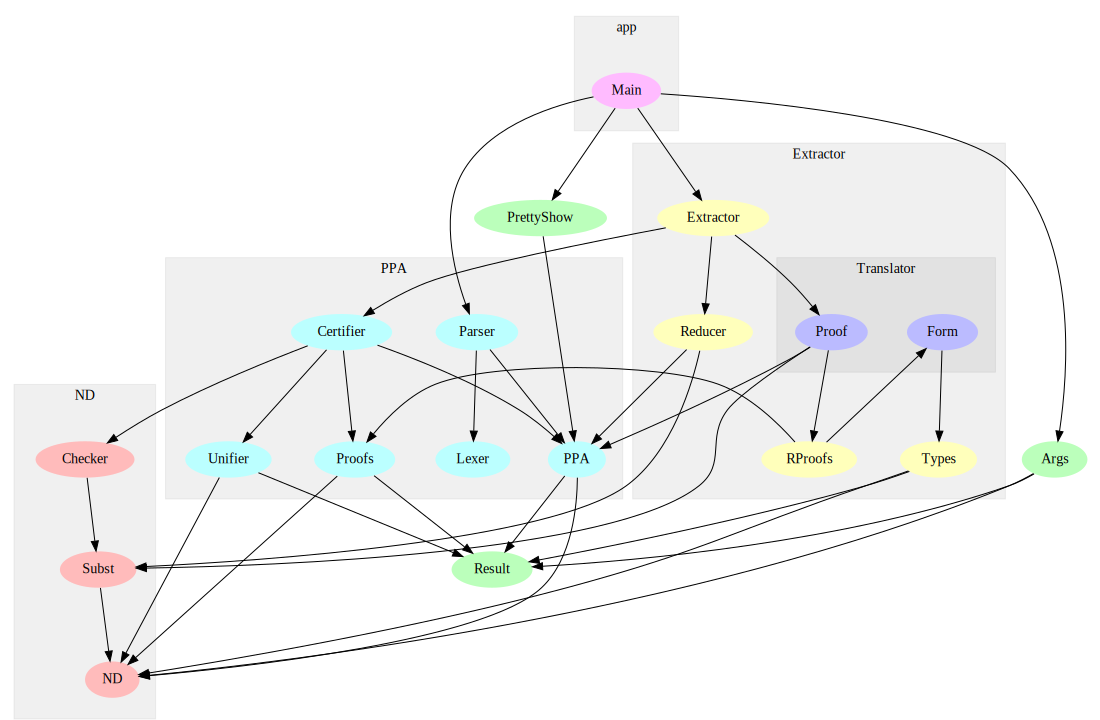
\includegraphics[scale=0.38]{img/modules.png}
    \caption{Grafo de módulos del programa \ppaTool{} generado con \href{https://github.com/yav/graphmod}{\texttt{graphmod}}}
\end{figure}

Los más relevantes son,

\begin{itemize}
    \item \texttt{ND}: Contiene el modelo central de deducción natural usado para los
    certificados. Fórmulas, términos y demostraciones. Tiene 3 sub módulos:
    \texttt{ND.Checker} (chequeador de demostraciones), \texttt{ND.Subst}
    (sustituciones sobre fórmulas y demostraciones) y \texttt{ND.ND} (el modelo
    en si). Ver \fullref{ppa-tool:sec:nd}.
    \item \texttt{PPA}: Contiene la implementación del lenguaje \ppaLang{} por
    sobre deducción natural.
    \begin{itemize}
        \item \texttt{PPA.Parser} y \texttt{PPA.Lexer} son el lexer y el parser
        respectivamente. Ver \fullref{ppa-tool:sec:parser-lexer}.
        \item \texttt{PPA.Certifier} implementa el certificador, que genera
        demostraciones de deducción natural a partir de programas de PPA. Usa
        \texttt{PPA.Unifier} para unificación (usado en eliminación de $\forall$) y \texttt{PPA.Proofs} para
        demostraciones de equivalencias en ND (usado en DNF).
    \end{itemize}
    \item \texttt{Extractor}: Contiene la lógica de extracción de testigos.
    Tiene varios sub módulos
    \begin{itemize}
        \item \texttt{Extractor.Translator} implementa la traducción de Friedman
        en sus dos sub-módulos, \texttt{Extractor.Translator.Proof} para
        demostraciones y\\\texttt{Extractor.Translator.Form} para fórmulas.
        \item \texttt{Extractor.Reducer} implementa la normalización.
        \item \texttt{Extractor.Extractor} combina todo lo anterior para hacer
        la extracción de testigos de principio a fin, certificando, traduciendo
        y reduciendo. Usa \\\texttt{Extractor.RProofs} que es análogo a
        \texttt{PPA.Proofs} e implementa los lemas necesarios sobre
        demostraciones intuicionistas con negación relativizada.
    \end{itemize}
\end{itemize}


\subsection{Parser y Lexer}
\label{ppa-tool:sec:parser-lexer}

Una parte esencial de \ppaTool{} es el compilador, que permite tomar un programa
desde un archivo de texto y llevarlo a una representación estructurada, como un
un tipo abstracto de datos, para el uso en el resto del programa. Se implementa
en dos etapas.

\begin{itemize}
    \item La primera es el análisis léxico o \textit{lexer}, que convierte el
    texto plano en una lista de \textit{lexemas} o \textit{tokens}. Se puede
    implementar con expresiones regulares.
    \item Una vez que el programa ya fue convertido en \textit{lexemas}, es
    procesado por el parser, que interpreta las estructuras sintácticas del
    lenguaje. Puede generar una representación intermedia como un tipo abstracto
    de datos.
\end{itemize}

Para el parsing en general hay dos caminos bien conocidos. O bien hacerlo a mano
con alguna biblioteca de \textit{parser combinators} como
\href{https://hackage.haskell.org/package/parsec}{parsec}, o usar un
\textit{parser generator}: un programa que genere un parser automáticamente a
partir de una gramática en algún formato como EBNF. Nosotros decidimos, por
familiaridad con el proceso, usar un parser generator. Los más conocidos
históricamente son Lex (para el lexer) y Yacc (para el parser, \textit{yet
another compiler compiler}). En Haskell existen dos paquetes análogos: \href{https://hackage.haskell.org/package/alex}{Alex} para el
lexer y \href{https://hackage.haskell.org/package/happy}{Happy} para el parser.
Estos generan un lexer a partir de expresiones regulares y un parser
respectivamente a partir de una gramática en un formato similar a EBNF.

En la \namedref{ppa-tool:fig:lexer} se puede ver un extracto del archivo de
input de Alex y en \namedref{ppa-tool:fig:parser} uno del de Happy de
\ppaTool{}. La implementación del parser solo construye términos de programas
(definidos en \texttt{PPA.PPA}) y fórmulas (\texttt{ND.ND}) a partir de los
cuales el programa opera.

\begin{figure}[p]
    \begin{minted}{text}
tokens :-
    $white+                         ;
    "//".*                          ; -- comments
    "/*"(.|(\r\n|\r|\n))*"*/"       ; -- block comments
    \.              { literal TokenDot }
    \,              { literal TokenComma }
    \&              { literal TokenAnd }
    \|              { literal TokenOr }
    true            { literal TokenTrue }
    false           { literal TokenFalse }
    \-\>            { literal TokenImp }
    \<\-\>          { literal TokenIff }
    \~              { literal TokenNot }
    exists          { literal TokenExists }
    forall          { literal TokenForall }
    \(              { literal TokenParenOpen }
    \)              { literal TokenParenClose }
    axiom           { literal TokenAxiom }
    theorem         { literal TokenTheorem }
    proof           { literal TokenProof }
    end             { literal TokenEnd }
    \;              { literal TokenSemicolon }
    \:              { literal TokenDoubleColon }
    suppose         { literal TokenSuppose }
    thus            { literal TokenThus }
    hence           { literal TokenHence }
    have            { literal TokenHave }
    then            { literal TokenThen }
    by              { literal TokenBy }
    equivalently    { literal TokenEquivalently }
    claim           { literal TokenClaim }
    cases           { literal TokenCases }
    case            { literal TokenCase }
    take            { literal TokenTake }
    \:\=            { literal TokenAssign }
    st              { literal TokenSuchThat }
    consider        { literal TokenConsider }
    let             { literal TokenLet }

    \"[^\"]*\"          { lex (TokenQuotedName . firstLast) }

    (\_|[A-Z])[a-zA-Z0-9\_\-]*(\')*                     { lex TokenVar }
    [a-zA-Z0-9\_\-\?!#\$\%\*\+\<\>\=\?\@\^]+(\')*       { lex TokenId }
    \end{minted}
    \caption{Extracto del lexer de \ppaTool{}}
    \label{ppa-tool:fig:lexer}
\end{figure}

\begin{figure}[p]
    \centering
    \begin{minted}{text}
%token
    -- Enumeración de tokens del lexer

Prog    : Declarations

Declarations : Declaration Declarations
                | Declaration

Declaration : Axiom
            | Theorem

Axiom : axiom Name ':' Form

Theorem : theorem Name ':' Form proof Proof end

Proof   : ProofStep Proof
        | {- empty -}

ProofStep : suppose Name ':' Form
            | thus Form OptionalBy
            | hence Form OptionalBy
            | have Name ':' Form OptionalBy
            | then Name ':' Form OptionalBy
            | equivalently Form
            | claim Name ':' Form proof Proof end
            | cases OptionalBy Cases end
            | take var ':=' Term
            | let var
            | consider var st Name ':' Form by Justification

Cases   : Case Cases
        | {- empty -}

Case    : case Form Proof
        | case Name ':' Form Proof

OptionalBy : by Justification
OptionalBy : {- empty -}

Justification : Name ',' Justification
                | Name

Name    : id
        | name

    \end{minted}
    \caption{Extracto del parser de \ppaTool{} (programas)}
    \label{ppa-tool:fig:parser}
\end{figure}

\begin{figure}[p]
    \begin{minted}{text}
-- Resolución automática de conflictos shift/reduce
%right exists forall dot
%right imp iff
%left and or
%nonassoc not
%%

Form    : id TermArgs
        | Form and Form
        | Form or Form
        | Form imp Form
        | Form iff Form
        | not Form
        | exists var dot Form
        | forall var dot Form
        | true
        | false
        | '(' Form ')'

Term    : var
        | id TermArgs

TermArgs : {- empty -}
            | '(' Terms ')'

Terms   : Term
        | Term ',' Terms
    \end{minted}
    \caption{Extracto del parser de \ppaTool{} (lógica de primer orden)}
    \label{ppa-tool:fig:parser-forms}
\end{figure}

\subsection{Modelado de deducción natural}
\label{ppa-tool:sec:nd}

La parte más interesante del modelado son las demostraciones de deducción
natural, que se pueden ver en la \namedref{ppa-tool:fig:nd-proofs}. Una
demostración está compuesta por la aplicación recursiva de reglas de inferencia,
y su modelo omite todos los detalles que se pueden inferir durante su chequeo.
De esa forma las demostraciones son más fáciles de escribir y generar, al costo
de ser un poco más costosas de leer por un humano, cosa que de todas formas no
deberíamos hacer. Por ejemplo, la introducción de la implicación, \ruleImpI{},
modelada por \texttt{PImpI} no especifica cuál es la implicación que se está
introduciendo, dado que durante el chequeo debería ser la fórmula actual a
demostrar. Tampoco se explicita en cada regla, cual es el contexto de
demostración. Se genera de forma dinámica.

\begin{figure}[p]
    \begin{multicols}{2}
    \begin{minted}{haskell}
    type VarId = String
    type FunId = String
    type PredId = String
    type HypId = String
    
    data Term
        = TVar VarId
        | TMetavar Metavar
        | TFun FunId [Term]
    
    data Form
        = FPred PredId [Term]
        | FAnd Form Form
        | FOr Form Form
        | FImp Form Form
        | FNot Form
        | FTrue
        | FFalse
        | FForall VarId Form
        | FExists VarId Form
    \end{minted}
    \end{multicols}
    \caption{Modelado de fórmulas y términos de LPO}
    \end{figure}
    

\begin{figure}[p]
\begin{multicols}{2}
\begin{minted}{haskell}
data Proof =
    | PAx HypId
    | PAndI
        { proofLeft :: Proof
        , proofRight :: Proof
        }
    | PAndE1
        { right :: Form
        , proofAnd :: Proof
        }
    | PAndE2
        { left :: Form
        , proofAnd :: Proof
        }
    | POrI1
        { proofLeft :: Proof
        }
    | POrI2
        { proofRight :: Proof
        }
    | POrE
        { left :: Form
        , right :: Form
        , proofOr :: Proof
        , hypLeft :: HypId
        , proofAssumingLeft :: Proof
        , hypRight :: HypId
        , proofAssumingRight :: Proof
        }
    | PImpI
        { hypAntecedent :: HypId
        , proofConsequent :: Proof
        }
    | PImpE
        { antecedent :: Form
        , proofImp :: Proof
        , proofAntecedent :: Proof
        }
    | PNotI
        { hyp :: HypId
        , proofBot :: Proof
        }
    | PNotE
        { form :: Form
        , proofNotForm :: Proof
        , proofForm :: Proof
        }
    | PTrueI
    | PFalseE
        { proofBot :: Proof
        }
    | PLEM
    | PForallI
        { newVar :: VarId
        , proofForm :: Proof
        }
    | PForallE
        { var :: VarId
        , form :: Form
        , proofForall :: Proof
        , termReplace :: Term
        }
    | PExistsI
        { inst :: Term
        , proofFormWithInst :: Proof
        }
    | PExistsE
        { var :: VarId
        , form :: Form
        , proofExists :: Proof
        , hyp :: HypId
        , proofAssuming :: Proof
        }
\end{minted}        
\end{multicols}
\caption{Modelado de reglas de inferencia para demostraciones}
\label{ppa-tool:fig:nd-proofs}
\end{figure}

\chapter{Conclusiones}

En este trabajo presentamos el lenguaje \ppaLang{} junto con los detalles de su
implementación en \ppaTool{}. Primero dimos una definición completa del sistema
lógico de deducción natural, junto con ejemplos de demostraciones. Describimos
cómo implementamos el algoritmo de chequeo, y por otro lado los de
alfa equivalencia y sustitución sin capturas en tiempo cuasilineal en peor caso.

Dimos un manual de usuario para el lenguaje \ppaLang{}, explicando como
escribir demostraciones y cómo usar el mecanismo de demostración principal
\lstinline{by}. Dimos una demostración completa que muestra diferentes capacidades del lenguaje. También se listaron
todos los comandos, ejemplos funcionales para cada uno, y su relación con las
reglas de inferencia de deducción natural. Profundizamos en la implementación
del certificador y cómo están implementadas cada una de las partes de la
interfaz. Centralmente el \textit{solver} usado por debajo del \lstinline{by}.

Finalmente vimos una implementación posible de extracción de testigos
existenciales. Mencionamos las limitaciones al tratar de hacerlo de forma
directa sobre lógica clásica, las distintas versiones de la traducción de
Friedman según el tipo de fórmula a demostrar, y las limitaciones que se
presentaron (no se podrá asumir cualquier axioma, ni demostrar cualquier fórmula
$\classPiTwo$). Luego describimos cómo a partir del isomorfismo Curry-Howard
pudimos implementar un mecanismo de normalización de demostraciones, que también
presentó limitaciones (no todas las demostraciones podrán ser llevadas a su
forma normal) y requirió cambios en la estrategia de reducción de una sencilla a
una más sofisticada (Gross-Knuth) debido al tamaño de las demostraciones.

El principal aporte del trabajo es la implementación práctica de un método de
extracción indirecto mediante el uso de la traducción de Friedman y la
normalización usual de la lógica intuicionista.

\section{Trabajo futuro}

Surgieron varias líneas de trabajo futuro, que quedaron fuera del alcance de la
tesis. Las listamos a continuación.

\begin{itemize}
    \item \textbf{Modelar de forma nativa inducción e igualdad}: las teorías que
    se pueden axiomatizar están limitadas al no poder representar inducción de
    forma nativa (como predica sobre predicados, es lógica de segundo orden). Si
    bien sí se puede axiomatizar de forma \textit{adhoc}, sería más amigable de
    estar como regla de inferencia y a lo largo de todo el programa. También se
    podría agregar de forma nativa la noción de \textit{igualdad}.
    \item \textbf{Sofisticar \textit{solver} del by}: en
    \fullref{ppa-cert:sec:expressiveness} se mencionan las limitaciones del
    \textit{solver} usado por el \lstinline{by}. Una funcionalidad que quedó
    afuera pero sería sencilla de agregar es que no solo se busque eliminar los
    $\forall$ consecutivos de \textit{una} hipótesis, sino que el proceso sea
    recursivo: que exhaustivamente intente de eliminar los $\forall$ de todas
    las combinaciones de hipótesis posibles.
    \item \textbf{Mejorar a PPA como lenguaje de programación}: el
    lenguaje PPA no brinda soporte para tener un ecosistema. Se pueden agregar
    muchas funcionalidades que mejorarían la calidad de vida del desarrollador
    como permitir importar archivos o módulos e implementar una biblioteca
    estándar de teorías y teoremas.
    \item \textbf{Extender PPA con tipos}: el lenguaje no permite ni especificar
    ni chequear tipos. Se podría implementar una versión tipada, basada en
    lógica de primer orden \textit{many sorted} (con varios géneros) que
    facilitaría la escritura de programas más sofisticados.
    \item \textbf{Refinar fórmulas \textit{conjuntivas}}: en la traducción de
    Friedman introducimos dos lemas centrales: $\formTwo \judgI \tdn{\formTwo}$
    \fullref{fri:lemma:trans-intro}, que vale para \textit{F-fórmulas}
    y restringe las axiomatizaciones, y $\fNotR
    \form \judgI \fNotR \tdn{\form}$ \fullref{fri:lemma:notr-trans-intro}, que
    vale para fórmulas \textit{conjuntivas}. Como el primero se reduce al
    segundo, podríamos refinar las fórmulas \textit{conjuntivas}, lo que
    permitiría usar más tipos de axiomas. También se podría profundizar en el
    vínculo con las fórmulas de Harrop mencionado en \namedref{fi:obs:harrop}.
    \item \textbf{Extender traducción de Friedman a más de un existencial}: en
    su versión final, lo máximo que llega a convertir son fórmulas de la forma
    $\forall \varTwo_1 \dots \forall \varTwo_n . \exists \var .
    \anyForm(\dots)$. Se debería poder extender a fórmulas de la forma $\forall
    \varTwo_1 \dots \forall \varTwo_n . \exists \var_1 \dots \exists \var_m .
    \anyForm(\dots)$.
    \item \textbf{Implementar versión completa de reducción de demostraciones}:
    en \fullref{fri:norm:sec:limitations} vimos las limitaciones del mecanismo
    de reducción implementado. Es ineficiente, y no se puede llegar a una forma
    normal útil para todas las demostraciones, evitando la extracción de
    testigos en casos donde debería ser posible. Se podrían extender para
    incluir reducciones permutativas e implementar una máquina abstracta para
    reducción \textit{call-by-need} o \textit{call-by-name}.
    \item \textbf{Mejorar reporte de errores}: los errores reportados por la
    herramienta en general son muy rústicos, implementativos y de bajo nivel. Se
    podrían hacer más amigables y accionables, ayudando a resolver problemas sin
    saber cómo funciona internamente la herramienta.
\end{itemize}

%%%% BIBLIOGRAFIA
\backmatter
\printbibliography

\end{document}